
%finisci l'ultimo doc

\documentclass[a4paper]{article}
\usepackage[utf8]{inputenc}
\usepackage{graphicx} % Required for inserting images
\usepackage[italian]{babel}
\usepackage{gensymb}
\usepackage{array}
\usepackage{amsmath}
\usepackage{hyperref}
\usepackage{siunitx}
\usepackage{placeins}
\usepackage[font=small,labelfont=bf]{caption}

\makeindex
\setlength{\parindent}{0pt}

\title{Misura dell'Accelerazione di Gravità usando un Pendolo}
\author{Francesco Giuliano Rossi}
\date{Marzo 2025}

\begin{document}
\maketitle
\tableofcontents

\newpage
\begin{abstract}
    L'obbiettivo di questo esperimento è di misurare l'accelerazione di gravità terrestre $g$ attraverso l'uso di un pendolo semplice. A tale scopo, si misurano periodi di oscillazioni per angoli piccoli (minore di 5\degree), per poi in seguito valutare gli effetti di angoli grandi e attriti.
\end{abstract}

\section{Introduzione Teorica}
\subsection{Il Pendolo Semplice}
L'esperimento si basa sull'uso del cosiddetto pendolo semplice, ovvero un punto materiale di massa $m$, appeso tramite un filo inestensibile, di lunghezza $l$ e di massa trascurabile. Per misurare le piccole oscillazioni, il corpo viene spostato dal punto di equilibrio e viene lasciato libero di oscillare. Dovuto al vincolo del filo inestensibile, il corpo è vincolato a seguire una traiettoria circolare a causa della tensione. Questo moto può essere schematizzato attraverso le equazioni di Newton:

\begin{equation} \label{Eq 1}
    \left\{
    \begin{array}{lr}
        ma_{c} = T - mg\cos\theta\\
        ma_{t} = -mg\sin\theta
    \end{array}
    \right.
\end{equation}

dove $a_{c}$ rappresenta l'accelerazione centripeta, e $a_{t}$ rappresenta quella tangenziale. Essendo un moto circolare, conviene passare a coordinati polari per una rappresentazione più semplice. Passando opportunamente a coordinate polari, con $a_{c} = l\dot{\theta}^2$ e $a_{t} = l\ddot{\theta}$, otteniamo un sistema di equazioni equivalente a (\ref{Eq 1}):

\begin{equation} \label{Eq 2}
    \left\{
    \begin{array}{lr}
        ml\dot{\theta} = T - mg\cos\theta \\
        ml\ddot{\theta} = -mg\sin\theta
    \end{array}
    \right.
\end{equation}

dove $l$ è la lunghezza del filo. Per piccole oscillazioni (di circa 5\degree), è possibile usare lo sviluppo in serie di Taylor $\sin\theta \approx \theta$, che fornisce l'equazione:

\begin{equation} \label{Eq 3}
    l\ddot{\theta} + g\theta = 0 \implies \ddot{\theta} + \frac{g}{l}\theta = 0
\end{equation}

anche noto come l'equazione del moto armonico. Una soluzione generale di questa equazione differenziale è data dalla equazione:

\begin{equation} \label{Eq 4}
    \theta(t) = \theta_{max}\sin({\omega t + \frac{\pi}{2}})
\end{equation}

dove $\omega = \sqrt{\frac{g}{l}}$, anche detto pulsazione del moto. Le costanti di integrazione (ampiezza massima e fase iniziale) si ottenono imponendo le condizioni iniziali di posizione e velocità: 

\begin{equation} \label{Eq 5}
    \left\{
        \begin{array}{lr}
            \theta(t=0) = \theta_{max} \\
            \dot{\theta}(t = 0) = 0
        \end{array}
    \right.
\end{equation}

mentre il periodi T delle piccole oscillazioni si ricava da:

\begin{equation} \label{Eq 6}
    \omega T = 2\pi \implies T = 2\pi \sqrt{\frac{l}{g}}
\end{equation}

Dalla (\ref{Eq 6}), risulta che la pulsazione non dipende dalla massa appesa, ma solo dall'accelerazione di gravità terrestre e la lunghezza del filo. A questo fenomeno viene dato il nome di isocronismo delle oscillazioni. Il modulo di $g$, usando quest'ultima equazione si potrà ricavare con l'equazione
\begin{equation}
    g = 4\pi^2 \frac{l}{T^2}
\end{equation}

\subsection{Il Pendolo Fisico}
Anche se il modello del pendolo semplice semplifica i calcoli, si può ottenere un modello migliore se consideriamo il pendolo fisico, ovvero un modello nel quale si approssima il filo a una barra rigida di massa $M_{f}$ e lunghezza $l_f$, e si sostituisce il punto materiale ad una sfera rigida di massa $M_{s}$, con raggio $r_s$. Scegliendo come polo il centro di rotazione $O$, il momento d'inerzia di tutto il sistema si può trovare considerando ogni componente del pendolo singolarmente, e sommando i risultati. Il momento d'inerzia per la massa (approssimando ad una sfera uniforme) è dato da:
\begin{equation}
    I_s = \frac{1}{2}\pi\int_{-r_s}^{r_s}{\frac{M_s}{\frac{4}{3}}\pi r^3_s}(r_s^2 - z^2)dz 
\end{equation}
Il momento d'inerzia del filo è dato da:

\begin{equation}
    I_f = \int_0^{l_f}{\frac{M_f}{l_f}x^2 dx}
\end{equation}

E il momento d'inerzia del centro di massa è dato da:
\begin{equation}
    I_{cms} = M_s({l_f}+r_s)^2
\end{equation}
Facendo il calcolo dei integrali, e sommando tutto si ottiene l'equazione del momento d'inerzia del sistema completo:
\begin{equation} \label{Eq 7}
    I = \frac{1}{3}M_f l^2_f +M_s(l_f+r_s)^2+\frac{2}{5}M_sr^2_s
\end{equation}

Questa equazione è stata trovata considerando il momento d'inerzia di ogni componente del pendolo e sommando i risultati. 
Rimanendo nell'approssimazione delle piccole oscillazioni, e assumendo le stesse condizioni iniziali di (\ref{Eq 4}), la traiettoria del sistema è descritta da:

\begin{equation} \label{Eq 8}
    \theta(t) = \theta_{max} \sin(\sqrt{\frac{mdg}{I}}t + \frac{\pi}{2}
\end{equation}

dove d è la distanza del centro di massa dal punto $O$ data dalla media pesata delle masse del filo e della sfera:

\begin{equation} \label{Eq 9}
    d = \frac{M_f\frac{l_f}{2} +M_s (l_f+R_s)}{M_f+M_s}
\end{equation}

Quindi il periodo sarà dato da:

\begin{equation} \label{Eq 10}
    T = \frac{2\pi}{\omega} = 2\pi\sqrt{\frac{I}{mdg}}
\end{equation}

Da cui si può ricavare l'equazione per g:

\begin{equation} \label{Eq 11}
    g = 4\pi^2\frac{I}{(M_f+M_s)T^2d}
\end{equation}

\section{Metodologia}
\subsection{Strumenti di Misura}
In laboratorio i strumenti che sono stati utilizzati sono:
\begin{itemize}
    \item Sfera usato come massa per il pendolo 
    \item Filo 
    \item Metro lineare con errore di sensibilità di \SI{5e-4}{\meter}
    \item Bilancia digitale con errore di sensibilità \SI{5e-6}{\kilogram}
    \item Calipro ventesimale digitale con errore di sensibilità \SI{5e-5}{\meter}
    \item Cronometro digitale \SI{1e-2}{\second}
\end{itemize}

\subsection{Procedimento}
Innanzitutto, è stata utilizzata la bilancia digitale per misurare il peso della sfera e il peso del filo. Dopodiché è stato utilizzato il calipro ventesimale per misurare il diametro della sfera e il metro lineare per misurare la lunghezza totale del filo. 
\newline Successivamente, la sfera è stata legata al filo e il sistema è stato appeso al pendolo. Un goniometro è stato posto sopra il centro di oscillazione per misurare il valore di $\theta$ iniziale. 
\newline Misurando dal centro di oscillazione fino al centro di massa del pendolo, Per ogni lunghezza (circa 0.30, 0.60, 1.20, 1.50, 1.80 metri) del filo sono stati prese 15 misure, mentre per la lunghezza di 1 metro abbiamo preso un totale di 100 misure, divisi in 10 set di dati. Poi, a partire da vari angoli di partenza (5\degree, 10\degree, 15\degree, 20\degree, 25\degree) sono stati presi 20 misure alla lunghezza di 1.50 metri. Infine, ad una lunghezza di 1.50 metri, si è fatto partire il pendolo da 30\degree, misurando (circa) ogni \SI{30}{second} il valore di $\theta$.

\subsection{Modi per Minimizzare l'Errore}
Per minimizzare l'errore nella ripresa dei dati, sono state adottate certe misure:
\begin{itemize}
    \item Prendere un totale di 5 oscillazioni per ogni misura, e facendo la media per calcolare un singolo periodo. In questo modo, l'errore relativo è minore, quindi risulta una maggiore precisione nella misura. 
    \item Usare come riferimento il passaggio sull'asse verticale piuttosto che nell'estremo. Risulta più semplice per l'occhio umano determinare la posizione di un oggetto in movimento piuttosto che quando inizia a muoversi.
\end{itemize}

\section{Risultati}
In seguito, saranno rapportati i risultati delle misure per ogni passo dello sperimento.
\subsection{Misure Varie Lunghezze Filo}
Riportate in seguito sono i risultati per le lunghezze di filo 0.282m, 0.587m, 1.209m, 1.802m. Le tabelle per 1.000m, e per 1.500m sono omesse e si trovano nelle sezioni \ref{Misura 1 metro} e \ref{Misura 1.50 metro}.
\begin{center}
    \begin{tabular}{|c|c|c|c|}
    \hline
    \multicolumn{4}{|c|}{$l=0.282$m} \\
    \hline
    5 Periodi(s) & Periodo Singolo(s) & 5 Periodi(s) & Periodo Singolo(s) \\
    \hline
     5.18 & 1.036 & 5.35 & 1.070 \\
     5.33 & 1.066 & 5.26 & 1.052 \\
     5.39 & 1.078 & 5.16 & 1.032 \\
     5.23 & 1.046 & 5.32 & 1.062 \\
     5.23 & 1.046 & 5.30 & 1.060 \\
     5.30 & 1.060 & 5.29 & 1.058 \\
     5.24 & 1.048 & 5.38 & 1.076 \\ 
     5.21 & 1.042 & & \\
    \hline
    \end{tabular}
\end{center}

\begin{center}
    \begin{tabular}{|c|c|c|c|}
    \hline
    \multicolumn{4}{|c|}{$l=0.587$m} \\
    \hline
    5 Periodi(s) & Periodo Singolo(s) & 5 Periodi(s) & Periodo Singolo(s) \\
    \hline
      7.64 & 1.528 & 7.72 & 1.544 \\
      7.66 & 1.532 & 7.67 & 1.534 \\
      7.66 & 1.532 & 7.67 & 1.534 \\
      7.61 & 1.522 & 7.60 & 1.520 \\
      7.66 & 1.532 & 7.61 & 1.522 \\
      7.63 & 1.526 & 7.66 & 1.532 \\
      7.58 & 1.516 & 7.63 & 1.526 \\ 
      7.56 & 1.512 &  & \\
    \hline
    \end{tabular}
\end{center}

\begin{center}
    \begin{tabular}{|c|c|c|c|}
    \hline
    \multicolumn{4}{|c|}{$l=1.209$m} \\
    \hline
    5 Periodi(s) & Periodo Singolo(s) & 5 Periodi(s) & Periodo Singolo(s) \\
    \hline
      11.00 & 2.200 & 11.12 & 2.224 \\
      11.06 & 2.212 & 11.15 & 2.230 \\
      11.03 & 2.206 & 11.13 & 2.226 \\
      11.06 & 2.12 & 11.01  & 2.202 \\
      11.06 & 2.12 & 11.07  & 2.14 \\
      11.05 & 2.210 & 11.00 & 2.200 \\
      11.07 & 2.214 & 11.00 & 2.200 \\ 
      11.11 & 2.222 & & \\
    \hline
    \end{tabular}
\end{center}

\begin{center}
    \begin{tabular}{|c|c|c|c|}
    \hline
    \multicolumn{4}{|c|}{$l=1.543$}\\
    \hline
    5 Periodi(s) & Periodo Singolo(s) & 5 Periodi(s) & Periodo Singolo(s) \\
    \hline
     12.60 & 2.520 & 12.46 & 2.492 \\
     12.52 & 2.504 & 12.47 & 2.492 \\
     12.55 & 2.510 & 12.43 & 2.486 \\
     12.54 & 2.508 & 12.48 & 2.496 \\
     12.44 & 2.488 & 12.45 & 2.484 \\
     12.55 & 2.510 & 12.50 & 2.500 \\
     12.40 & 2.480 & 12.44 & 2.488 \\
     12.41 & 2.482 & & \\
    \hline
    \end{tabular}
\end{center}

\begin{center}
    \begin{tabular}{|c|c|c|c|}
    \hline
    \multicolumn{4}{|c|}{$l=1.802$m} \\
    \hline
    5 Periodi(s) & Periodo Singolo(s) & 5 Periodi(s) & Periodo Singolo(s) \\
    \hline
     13.40 & 2.680 & 13.47 & 2.694 \\
     13.49 & 2.698 & 13.43 & 2.686 \\
     13.43 & 2.686 & 13.47 & 2.694 \\
     13.42 & 2.684 & 13.43 & 2.686 \\
     13.44 & 2.688 & 13.52 & 2.704 \\
     13.52 & 2.704 & 13.38 & 2.676 \\
     13.50 & 2.700 & 13.48 & 2.696 \\ 
     13.43 & 2.686 & & \\
    \hline
    \end{tabular}
\end{center}

\subsection{Misure con Filo di 1 Metro} \label{Misura 1 metro}
In seguito sono rapportati i dati, raggruppati in set di 10 misure, tutte effettuate con una lunghezza di $l=99.1$m.
\begin{center}
    \tabcolsep=0.11cm
    \begin{tabular}{|c|c||c|c|}
    \hline
    \multicolumn{2}{|c||}{Oscillazioni 1-10} & \multicolumn{2}{|c|}{Oscillazioni 11-20} \\
    \hline
    5 Periodi(s) & T Singolo(s) & 5 Periodi(s) & T Singolo(s) \\
    \hline
      10.01 & 2.002 & 10.00 & 2.000 \\
      10.00 & 2.000 & 10.06 & 2.012\\
      10.01 & 2.002 & 10.03 & 2.006\\
      10.03 & 2.006 & 10.00 & 2.00\\
      10.06 & 2.012 & 10.02 & 2.004\\
      10.00 & 2.000 & 10.03 & 2.006\\
      10.07 & 2.014 & 10.00 & 2.00\\ 
      10.01 & 2.002 & 10.07 & 2.014\\
      10.01 & 2.002 & 10.01 & 2.002\\
      10.03 & 2.006 &  9.98 & 1.996\\
    \hline
    \end{tabular}
\end{center}

\begin{center}
    \begin{tabular}{|c|c||c|c|}
    \hline
    \multicolumn{2}{|c||}{Oscillazioni 21-30} & \multicolumn{2}{|c|}{Oscillazioni 31-40} \\
    \hline
    5 Periodi(s) & T Singolo(s) & 5 Periodi(s) & T Singolo(s) \\
    \hline
      10.03 & 2.006 & 10.08 & 2.016 \\
      10.01 & 2.002 &  9.93 & 1.986\\
       9.95 & 1.990 &  9.96 & 1.992\\
       9.96 & 1.992 &  9.93 & 1.986 \\
       9.93 & 1.986 & 10.00 & 2.000\\
      10.01 & 2.002 & 10.01 & 2.002\\
      10.03 & 2.006 &  9.98 & 1.996\\ 
       9.93 & 1.986 &  9.96 & 1.992\\
      10.01 & 2.002 &  9.98 & 1.996\\
      10.10 & 2.020 & 10.06 & 2.012\\
    \hline
    \end{tabular}
\end{center}

\begin{center}
    \begin{tabular}{|c|c||c|c|}
    \hline
    \multicolumn{2}{|c||}{Oscillazioni 41-50} & \multicolumn{2}{|c|}{Oscillazioni 51-60} \\
    \hline
    5 Periodi(s) & T Singolo(s) & 5 Periodi(s) & T Singolo(s) \\
    \hline
      10.04 & 2.008 &  9.96 & 1.992 \\
      10.03 & 2.006 & 10.01 & 2.002 \\
      10.03 & 2.006 & 10.03 & 2.006 \\
       9.96 & 1.992 &  9.89 & 1.978 \\
      10.01 & 2.002 & 10.01 & 2.002 \\
       9.90 & 1.980 & 10.00 & 2.000 \\
      10.04 & 2.008 & 10.09 & 2.018 \\ 
       9.97 & 1.994 & 10.01 & 2.002 \\
       9.90 & 1.980 & 10.04 & 2.008 \\
       9.91 & 1.982 & 10.06 & 2.001 \\
    \hline
    \end{tabular}
\end{center}

\begin{center}
    \begin{tabular}{|c|c||c|c|}
    \hline
    \multicolumn{2}{|c||}{Oscillazioni 61-70} & \multicolumn{2}{|c|}{Oscillazioni 71-80} \\
    \hline
    5 Periodi(s) & T Singolo(s) & 5 Periodi(s) & T Singolo(s) \\
    \hline
      10.13 & 2.026 &  9.95 & 1.990 \\
       9.89 & 1.978 &  9.91 & 1.982 \\
       9.95 & 1.990 & 10.09 & 2.018 \\
       9.97 & 1.994 & 10.01 & 2.002 \\
       9.90 & 1.980 &  9.89 & 1.978 \\
      10.03 & 2.006 & 10.04 & 2.008 \\
      10.07 & 2.014 &  9.95 & 1.990 \\ 
      10.01 & 2.002 & 10.01 & 2.002 \\
       9.96 & 1.992 & 10.00 & 2.000 \\
      10.01 & 2.002 & 10.01 & 2.002 \\
    \hline
    \end{tabular}
\end{center}

\begin{center}
    \begin{tabular}{|c|c||c|c|}
    \hline
    \multicolumn{2}{|c||}{Oscillazioni 81-90} & \multicolumn{2}{|c|}{Oscillazioni 91-100} \\
    \hline
    5 Periodi(s) & T Singolo(s) & 5 Periodi(s) & T Singolo(s) \\
    \hline
      10.04 & 2.008 &  9.87 & 1.974 \\
       9.96 & 1.992 &  9.95 & 1.990 \\
      10.01 & 2.002 & 10.02 & 2.004 \\
      10.00 & 2.000 &  9.89 & 1.978 \\
       9.92 & 1.984 & 10.00 & 2.000 \\
       9.93 & 1.986 &  9.87 & 1.974 \\
      10.04 & 2.008 & 10.00 & 2.000 \\ 
       9.93 & 1.986 &  9.98 & 1.996 \\
       9.90 & 1.980 &  9.96 & 1.992 \\
      10.00 & 2.000 & 10.09 & 2.018 \\
    \hline
    \end{tabular}
\end{center}

\subsection{Misure con Angoli di Partenza Diversi} \label{Misura 1.50 metro}
In seguito, sono rapportati i dati misurati con una lunghezza di $l=1.543$m, partendo da diversi angoli di $\theta$.

\begin{center}
    \begin{tabular}{|c|c|c|c|}
    \hline
    \multicolumn{4}{|c|}{$\theta=5\degree$} \\
    \hline
    5 Periodi(s) & T Singolo(s) & 5 Periodi(s) & T Singolo(s) \\
    \hline
     12.60 & 2.520 & 12.43 & 2.486 \\
     12.52 & 2.504 & 12.48 & 2.496 \\
     12.55 & 2.510 & 12.45 & 2.484 \\
     12.54 & 2.508 & 12.50 & 2.500 \\
     12.44 & 2.488 & 12.44 & 2.488 \\
     12.55 & 2.510 & 12.52 & 2.504 \\
     12.40 & 2.480 & 12.42 & 2.484 \\
     12.41 & 2.482 & 12.47 & 2.494 \\
     12.47 & 2.494 & 12.48 & 2.496 \\
     12.46 & 2.492 & 12.43 & 2.486 \\
    \hline
    \end{tabular}
\end{center}

\begin{center}
    \begin{tabular}{|c|c|c|c|}
    \hline
    \multicolumn{4}{|c|}{$\theta=10\degree$} \\
    \hline
    5 Periodi(s) & T Singolo(s) & 5 Periodi(s) & T Singolo(s) \\
    \hline
    12.55 & 2.510 & 12.58 & 2.516 \\
    12.50 & 2.500 & 12.48 & 2.492 \\
    12.51 & 2.502 & 12.59 & 2.492 \\
    12.57 & 2.492 & 12.56 & 2.484 \\
    12.58 & 2.486 & 12.56 & 2.512 \\
    12.56 & 2.492 & 12.49 & 2.486 \\
    12.59 & 2.506 & 12.53 & 2.506 \\
    12.53 & 2.482 & 12.46 & 2.488 \\
    12.50 & 2.500 & 12.48 & 2.496 \\
    12.49 & 2.498 & 12.53 & 2.506 \\
    \hline
    \end{tabular}
\end{center}

\begin{center}
    \begin{tabular}{|c|c|c|c|}
    \hline
    \multicolumn{4}{|c|}{$\theta=15\degree$} \\
    \hline
    5 Periodi(s) & T Singolo(s) & 5 Periodi(s) & T Singolo(s) \\
    \hline
    12.56 & 2.512 & 12.55 & 2.510 \\
    12.55 & 2.510 & 12.55 & 2.488 \\
    12.59 & 2.488 & 12.48 & 2.492 \\
    12.58 & 2.498 & 12.53 & 2.506 \\
    12.62 & 2.492 & 12.48 & 2.496 \\
    12.52 & 2.504 & 12.51 & 2.500 \\
    12.60 & 2.520 & 12.50 & 2.492 \\
    12.55 & 2.510 & 12.56 & 2.512 \\
    12.60 & 2.520 & 12.55 & 2.511 \\
    12.56 & 2.515 & 12.55 & 2.511 \\
    \hline
    \end{tabular}
\end{center}

\begin{center}
    \begin{tabular}{|c|c|c|c|}
    \hline
    \multicolumn{4}{|c|}{$\theta=20\degree$} \\
    \hline
    5 Periodi(s) & T Singolo(s) & 5 Periodi(s) & T Singolo(s) \\
    \hline
    12.64 & 2.528 & 12.61 & 2.522 \\
    12.63 & 2.526 & 12.53 & 2.506 \\
    12.60 & 2.520 & 12.55 & 2.510 \\
    12.62 & 2.524 & 12.58 & 2.516 \\
    12.60 & 2.520 & 12.53 & 2.506 \\
    12.64 & 2.528 & 12.57 & 2.514 \\
    12.61 & 2.522 & 12.56 & 2.512 \\
    12.63 & 2.526 & 12.58 & 2.516 \\
    12.55 & 2.510 & 12.62 & 2.524 \\
    12.57 & 2.514 & 12.63 & 2.526 \\
    \hline
    \end{tabular}
\end{center}

\begin{center}
    \begin{tabular}{|c|c|c|c|}
    \hline
    \multicolumn{4}{|c|}{$\theta=25\degree$} \\
    \hline
    5 Periodi(s) & T Singolo(s) & 5 Periodi(s) & T Singolo(s) \\
    \hline
    12.63 & 2.526 & 12.67 & 2.534 \\
    12.68 & 2.536 & 12.63 & 2.526 \\
    12.61 & 2.522 & 12.60 & 2.520 \\
    12.63 & 2.526 & 12.56 & 2.512 \\
    12.56 & 2.512 & 12.61 & 2.522 \\
    12.58 & 2.516 & 12.61 & 2.522 \\
    12.61 & 2.522 & 12.63 & 2.526 \\
    12.62 & 2.524 & 12.70 & 2.540 \\
    12.56 & 2.512 & 12.58 & 2.516 \\
    12.65 & 2.530 & 12.64 & 2.528 \\
    \hline
    \end{tabular}
\end{center}

\subsection{Misure di $\theta$ per Attriti}
In seguito, sono rapportati i dati di $\theta$, misurati circa ogni 30 secondi, dopo che il pendolo è stato lasciato con un angolo iniziale di 30\degree.

\begin{center}
    \begin{tabular}{|c|c|}
    \hline
    $\theta_{max}$ & Tempo (s) \\
    \hline
     30\degree & 000.00 \\
     22\degree & 031.09 \\
     19\degree & 060.07 \\
     16\degree & 090.38 \\
     13\degree & 121.36 \\
     11\degree & 151.38 \\
     10\degree & 182.59 \\
     9\degree  & 210.23 \\
     8\degree  & 243.79 \\
     7\degree  & 272.49 \\
     6\degree  & 298.99 \\
    \hline
    \end{tabular}
\end{center}

\section{Analisi dei Dati}
\subsection{Calcolo del Valore di G}
Riportato nella seguente tabella, sono i valori medi trovati per il periodo per le varie lunghezze del pendolo con le varianze sulla misura, e il valore di g calcolato e la varianza su di g.

\begin{center}
    \begin{tabular}{|c|c|c|c|c|}
    \hline
    $l$ (m) & $\bar{T}$ (s)& $\sigma_{\bar{T}}$ (s) & Valore di $g$ (m/s$^2$)& $\sigma_g$  (m/s$^2$)\\
    \hline
      0.282 & 1.056 & $\pm{0.004}$& 10.00 & $\pm{0.077}$\\
      0.587 & 1.527 & $\pm{0.002}$& 9.938 & $\pm{0.026}$\\
      0.991 & 1.999 & $\pm{0.001}$& 9.791& $\pm{0.030}$\\
      1.209 & 2.212 & $\pm{0.002}$& 9.755 & $\pm{0.018}$\\
      1.543 & 2.497 & $\pm{0.003}$& 9.778 & $\pm{0.024}$\\
      1.802 & 2.691 & $\pm{0.002}$& 9.824 & $\pm{0.022}$\\
    \hline
    \end{tabular}
\end{center}

Calcolando le medie pesate, sugli errori, si calcola un'accelerazione di gravità pari a:
\begin{equation}
    g = 9.810 \SI{\pm0.010}{m/s^2}
\end{equation}

\subsection{Dipendenza di $T$ da $l$}
Si vuole verificare graficamente se i dati raccolti possono seguire certe relazioni. Si deve verificare l'andamento per vari possibili relazioni, come $T=al$, $T=al^2$, $T=al^\frac{1}{2}$, $T=al^\frac{3}{2}$. Si assumerà che la relazione $T=al^\frac{1}{2}$ sia la relazione migliore in accordo con i dati, e usando questa relazione si stima il parametro T con il metodo grafico e si verifica la compatibilità dei valori misurati con l'ipotesi. Inoltre, si fa un grafico $T-l^\alpha$, dove $\alpha$ sono le rispettive potenze e si verifica visivamente che solo quando $\alpha = 2$ si ha una retta, confermando la teoria vista prima.

\subsection{Confronto con il Pendolo Fisico}
Per questa sezione si usa il modello proposto nella sezione 1.2. Sono importante le misure della massa del filo, la massa della sfera, raggio della sfera e lunghezza totale del filo, rapportati nella seguente tabella

\begin{center}
    \begin{tabular}{|c|c|c|c|}
    \hline
    Massa Filo(kg)&Massa Sfera(kg)&Raggio Sfera(m) & Lunghezza filo(m)\\
    \hline
    0.00131 & 0.05297 & 0.02093 & 1.97 \\

    \hline
    \end{tabular}
\end{center}
Usando questi dati si può procedere con il calcolo di $g$. Rapportati, sono i valori di $g$ calcolati usando tale modello. 
\begin{center}
    \begin{tabular}{|c|c|c|}
    \hline
    Lunghezza filo & Valore di $g_f$ & Differenza con $g_s$\\
    \hline
    0.282 & 9.961 & 0.039\\
    0.587 & 9.902 & 0.036\\
    0.991 & 9.752 & 0.039\\
    1.209 & 9.716 & 0.039\\
    1.543 & 9.730 & 0.048\\
    1.802 & 9.777 & 0.047\\
    \hline
    \end{tabular}
\end{center}
come possiamo vedere, tutte queste misure sono entro tre $\sigma_g$, e quindi compatibili con le misure ottenute con il pendolo semplice. Questo sopporta l'ipotesi che la modellazione del pendolo semplice è valida come approssimazione.

\subsection{Attriti}
È molto importante valutare gli attriti per vedere se si possono trascurare o meno nella fase di analisi dei dati. Per questo si misura la variazione dell'ampiezza massima in un arco di tempo pari a 5 minuti. Partendo dall'ampiezza iniziale $\theta_{max} = 30\degree$ si può usare l'equazione oraria che descrive il moto del sistema
\begin{equation}
    \theta (t) = \theta_{max} e^{-\frac{t}{\tau_A}}
\end{equation}
e applicando l'equazione ai diversi $t_i$ e i valori $\theta_{max} (t_i)$ si può ricavare una espressione per $\tau_A$
\begin{equation}
    \tau_A = \frac{t_i}{ln{\frac{\theta_{max}}{\theta_{max} (t_i)}}}
\end{equation}
Facendo un grafico di 
\begin{equation}
    \ln{\frac{\theta_{max}}{\theta_{max}(t_i)}} = y = mx = (\frac{1}{\tau_A})t
\end{equation}
dove si ha $t$ in ascissa e $\ln{\frac{\theta_{max}}{\theta_{max}(t_i)}}$ in ordinata, e calcolando il coefficiente angolare si ottiene l'inverso di $\tau_A$. Per la tabella con le misure si guarda la sezione 3.4. Per i grafici si guarda la sezione 5.2. Facendo il grafico, e trovando la retta che stima nel modo migliore i dati, si ottiene un $\tau_a = 3 \text{ minuti e }  21 \text{ secondi}$. 

\subsection{Oltre le Piccole Oscillazioni (Dipendenza di T da $\theta_{max}$)}
In questa sezione si vuole dimostrare che l'approssimazione fatta nel pendolo semplice vale solo per angoli piccoli. Per verificare questo, si fa partire il pendolo da un angolo di $\theta = 30\degree$ e si misura l'angolo massimo ogni 30 secondi. In questo modo si può verificare se le formule usate per calcolare g valgono solo per angoli piccoli. Nella sezione 1.1, viene usato l'approssimazione $\sin x \approx x$, tuttavia per angoli grandi questa approssimazione non vale. Imponendo la conservazione dell'energia meccanica, scegliendo lo $0$ come la quota zero del potenziale si ottiene un periodo per angoli grandi di 
\begin{equation}
    T = 2\pi \sqrt{\frac{l}{g}} [1+\frac{1}{4}\sin^2 \frac{\theta_{max}}{2} + \frac{9}{64}\sin^4 \frac{\theta_{max}}{2}+...]
\end{equation}
posto $S(\theta_{max}) = 1+\frac{1}{4}\sin^2 \frac{\theta_{max}}{2} + \frac{9}{64}\sin^4 \frac{\theta_{max}}{2}+...$, questa espressione è equivalente a 

\begin{equation}
    T = T_0 S(\theta_{max})
\end{equation}
In questo modo, usando i dati rapportati nelle tabelle della sezione, 3.3, si ottengono i risultati:

\begin{center}
    \begin{tabular}{|c|c|c|c|c|}
    \hline
   $\theta(t_0)$ & $\bar{T}$ & $\sigma_{\bar{T}}$ & $S(\theta_{max})$ & $T_0 S(\theta_{max})$ \\
    \hline
       5$\degree$ & 2.496 & 0.002 & 1.000476 & 2.498 \\
      10$\degree$ & 2.506 & 0.002 & 1.001907 & 2.511 \\
      15$\degree$ & 2.509 & 0.002 & 1.004300 & 2.520 \\
      20$\degree$ & 2.517 & 0.002 & 1.007666 & 2.536 \\
      25$\degree$ & 2.519 & 0.002 & 1.012020 & 2.549 \\
    \hline
    \end{tabular}
\end{center}

Facendo il grafico di $S(\theta_{max}) \text{vs} \bar{T}$, si ottiene in coefficiente lineare di $1.84\pm{0.43}$, il che è entro $3\sigma$ del valore di $T_0 = 2\pi \sqrt{\frac{l}{g}} \approx \SI{2.50}{s}$. 
Come si può osservare nella tabella, le misure di $T_0 S(\theta_{max})$, fino a $10\degree$ rientrano in $3\sigma_{\bar{T}}$, ma dopo $10\degree$, non rientrano più in questo intervallo. Questo ci dà una buona indicazione che l'approssimazione delle piccole oscillazioni è valida solo quando si prende un angolo meno di $10\degree$. Questo potrebbe essere dato da vari fattori come il modo che è costruito il sopporto, o anche dovuto al attrito dell'aria. 

\subsection{Confronto Istogramma-Gaussiana}
Alla lunghezza $l=0.991m$, sono state effettuate 100 misure che mettendo in un istogramma, si riconosce che formano una distribuzione normale o Gaussiana. La funzione Gaussiana è una distribuzione di probabilità che si basa sui parametri $\mu$ e $\sigma^2$. L'equazione della Gaussiana è:
\begin{equation}
    f(x)=N(\hat{\mu}, \hat{\sigma}^2) = \frac{1}{\sqrt{2\pi}\hat{\sigma}}\exp{-\frac{(x-\hat{\mu}^2)}{2\hat{\sigma}^2}}
\end{equation}
La miglior stima dei parametri è data dal metodo del maximum likelihood, che dice che la miglior stima del parametro $\mu$ è quello che massimizza la funzione di likelihood. Questo valore risulta essere 
\begin{equation}
    \hat{\mu} = \frac{1}{n} \sum_{i=1}^{n}\tau_i = 9.99s
\end{equation}
e quindi la miglior stima della varianza $\hat{\sigma^2}$ risulta essere 
\begin{equation}
    \hat{\sigma}^2 = \frac{1}{n-1} \sum_{i=1}^{n}(\tau_i - \hat{\mu})^2
\end{equation}
e quindi la miglior stima della deviazione standard risulta essere 
\begin{equation}
    \hat{\sigma} = \sqrt{\hat{\sigma}^2} = \sqrt{\frac{1}{n-1} \sum_{i=1}^{n}(\tau_i - \hat{\mu})^2} = 0.056
\end{equation}
Usando la distribuzione di Gauss, con questi valori, è possibile ricavare il numero di eventi attesi $n_k^c$ nel k-esimo intervallo $\Delta x_k$, dato dalla relazione 
\begin{equation}
    n^c_k = n_{tot} P_k = n_{tot} \Delta x_k f(\bar{x_k})
\end{equation}
dove $P_k$ è la probabilità che un evento si trovi nel k-esimo intervallo, $\Delta x_k$, rappresenta la larghezza del singolo intervallo, $f(\bar{x_k})$ è la funzione Gaussiana valutata nel punto medio di ciascun intervallo, e $n_tot$ è il numero totale di misure effettuate. Questo valore teorico va confrontato con il valore misurato $n^m_k$, così che si possono confrontare i valore ottenuti sperimentalmente e quelli teorici. Sapendo che la Gaussiana è la distribuzione binomiale, ma per $n_{tot} >> n_k^c$, la deviazione standard risulta essere 
\begin{equation}
    \sigma_{n_k} = \sqrt{n_{tot}P_i(1-P_i)} = \sqrt{n^c_k (1-\frac{n_k^c}{n_tot})} \approx n^c_k
\end{equation}
Affinché le misure sono compatibili, i valori attesi devono essere entro tre deviazioni standard dei valori misurati, ovvero deve essere verificata l'uguaglianza 
\begin{equation}
    |n^m_k - n^c_k| < 3\sigma_{n_k}
\end{equation}
Usando i valori per i vari intervalli, si ottiene: 
\begin{center}
\begin{tabular}{|c|c|c|c|c|}
\hline
Intervalli & Valore Medio & Eventi Misurati & Eventi attesi & $\sigma$ \\ 
\hline
1          & 9.87-9.90    & 6               & 3.32          & 1.77                \\ 
2          & 9.90-9.93    & 7               & 8.08          & 2.73                \\ 
3          & 9.93-9.96    & 11              & 14.78         & 3.55                \\ 
4          & 9.96-9.99    & 14              & 20.28         & 4.02                \\ 
5          & 9.99-10.02   & 32              & 20.89         & 4.07                \\ 
6          & 10.02-10.05  & 18              & 16.15         & 3.68                \\ 
7          & 10.05-10.08  & 7               & 9.37          & 2.91                \\ 
8          & 10.08-10.11  & 5               & 4.08          & 1.98                \\ 
9          & 10.11-10.14  & 1               & 1.334         & 1.15                \\ \hline
\end{tabular}
\end{center}

\section{Conclusione}
Come si può osservare, il valore finale calcolato di $g=\SI{9.810}{m/s^2}$, che è entro $3\sigma$ del valore accettato per Trieste, $g_t=\SI{9.807}{m/s^2}$. 

L'errore più grande in questo esperimento è il fattore umano nella registrazione del tempo. Questo fattore potrebbe essere minimizzato prendendo più misure, così avendo più dati, si può avere una misura più precisa. Inoltre, la tensione del filo durante l'oscillazione del pendolo cambia in base al punto in cui si trova. Essendo più teso il filo il momento in cui il pendolo passa per la verticale, c'è un piccolo allungamento del filo. Se si tiene conto di queste due considerazioni, si potrebbe ottenere una misura più accurata. 

\newpage
\section{Figure}
\subsection{Istogrammi}
\subsubsection{Istogrammi lunghezze diverse}
\begin{figure}[!h]
    \centering
    \begin{minipage}[b]{0.4\textwidth}
      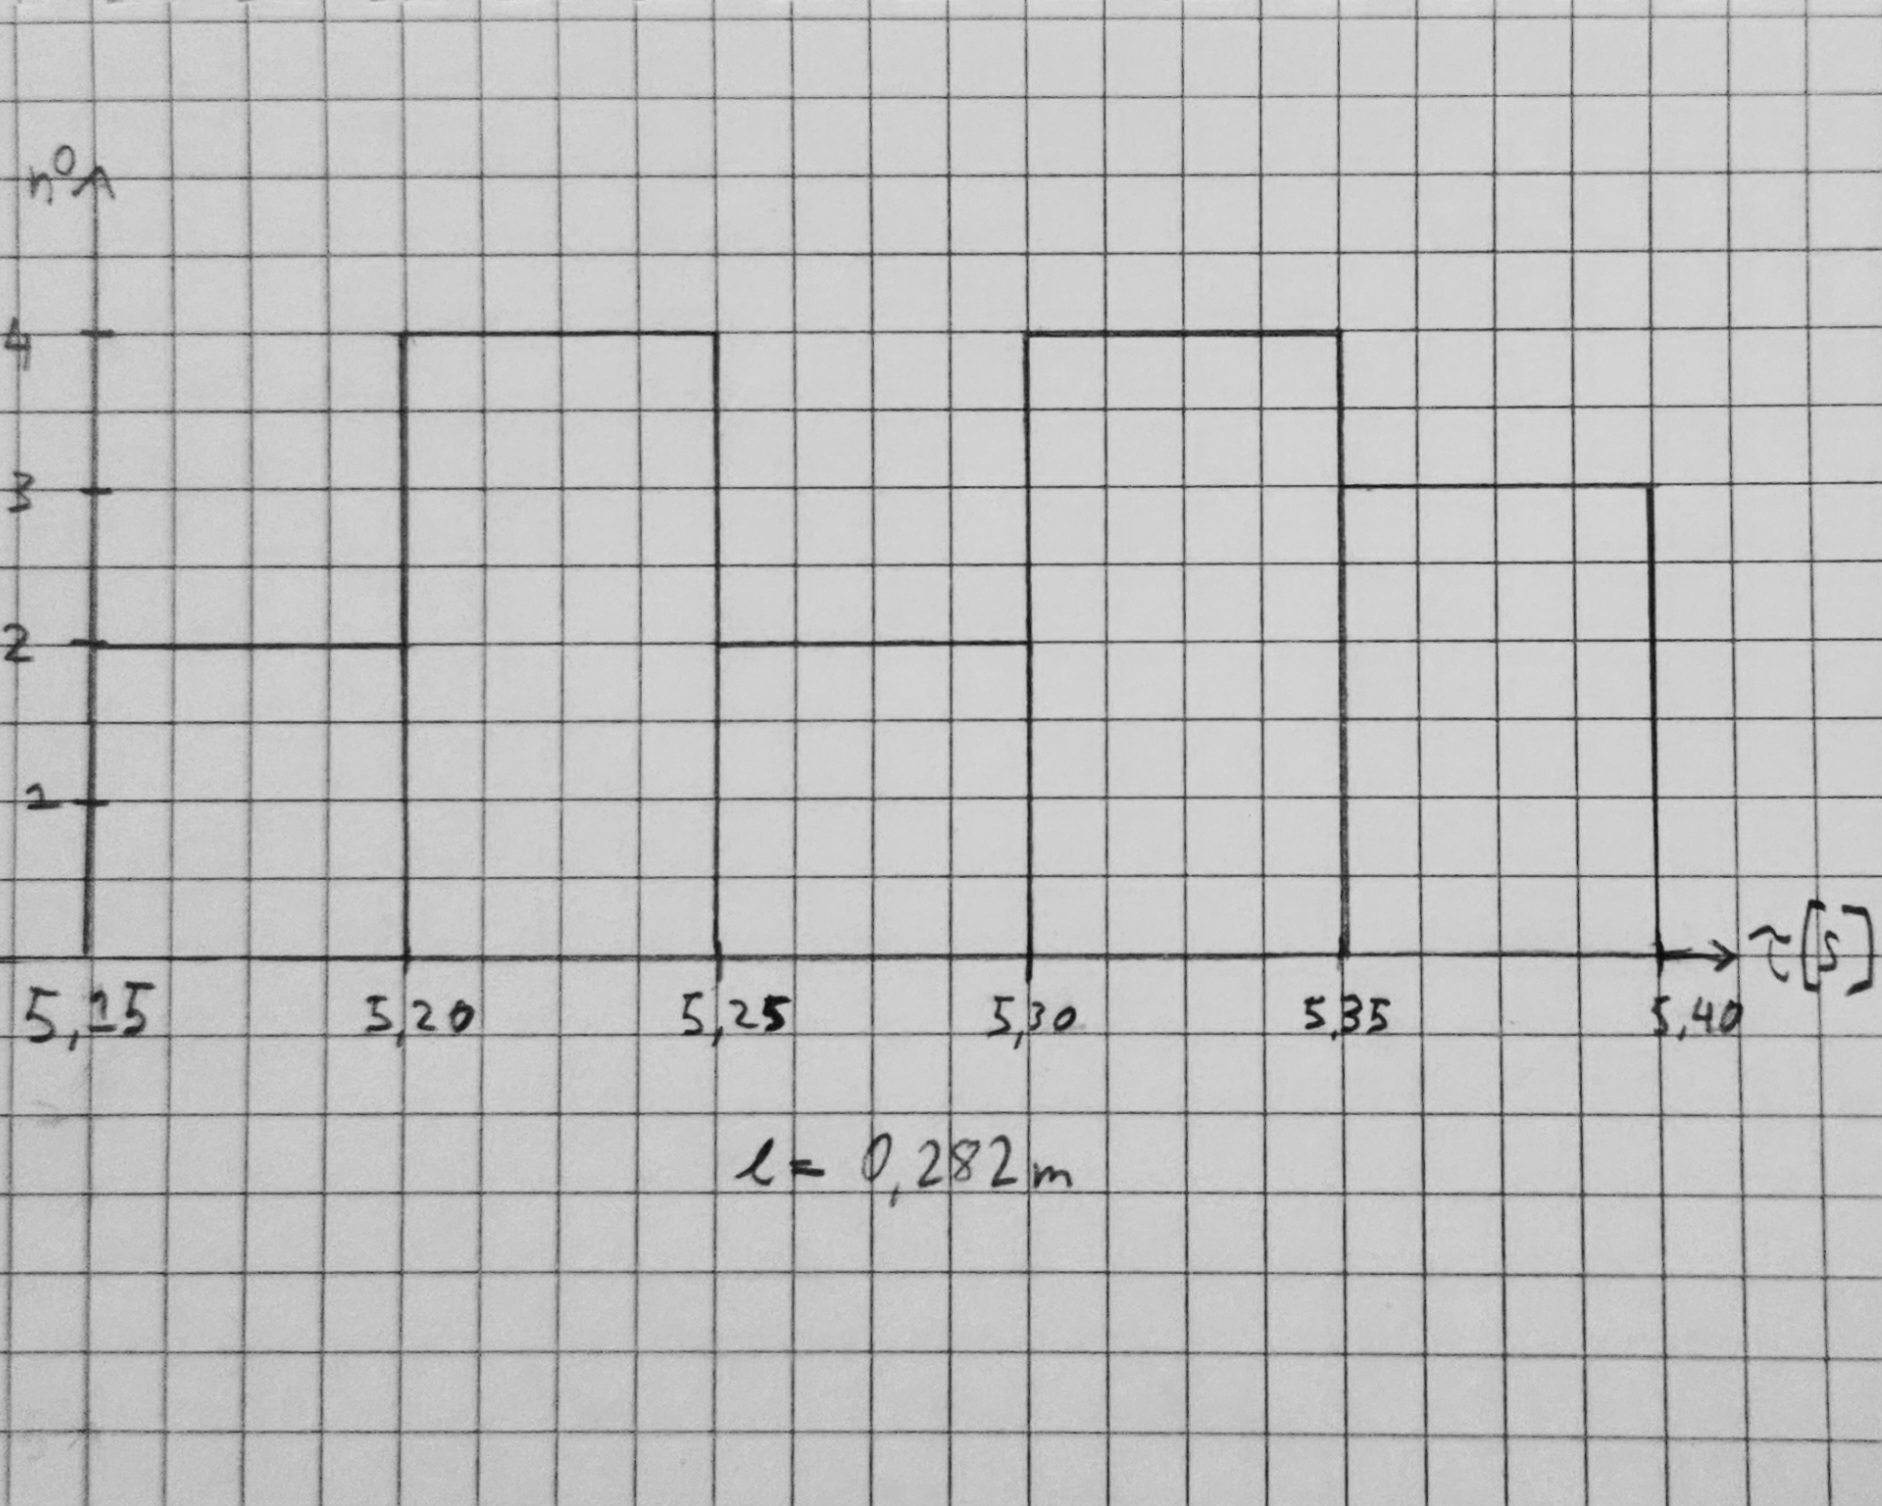
\includegraphics[width=\textwidth]{fotopendolo/lunghezza_0282.jpg}
      \caption{Misure con $l=0.282m$}
    \end{minipage}
    \hfill
    \begin{minipage}[b]{0.4\textwidth}
      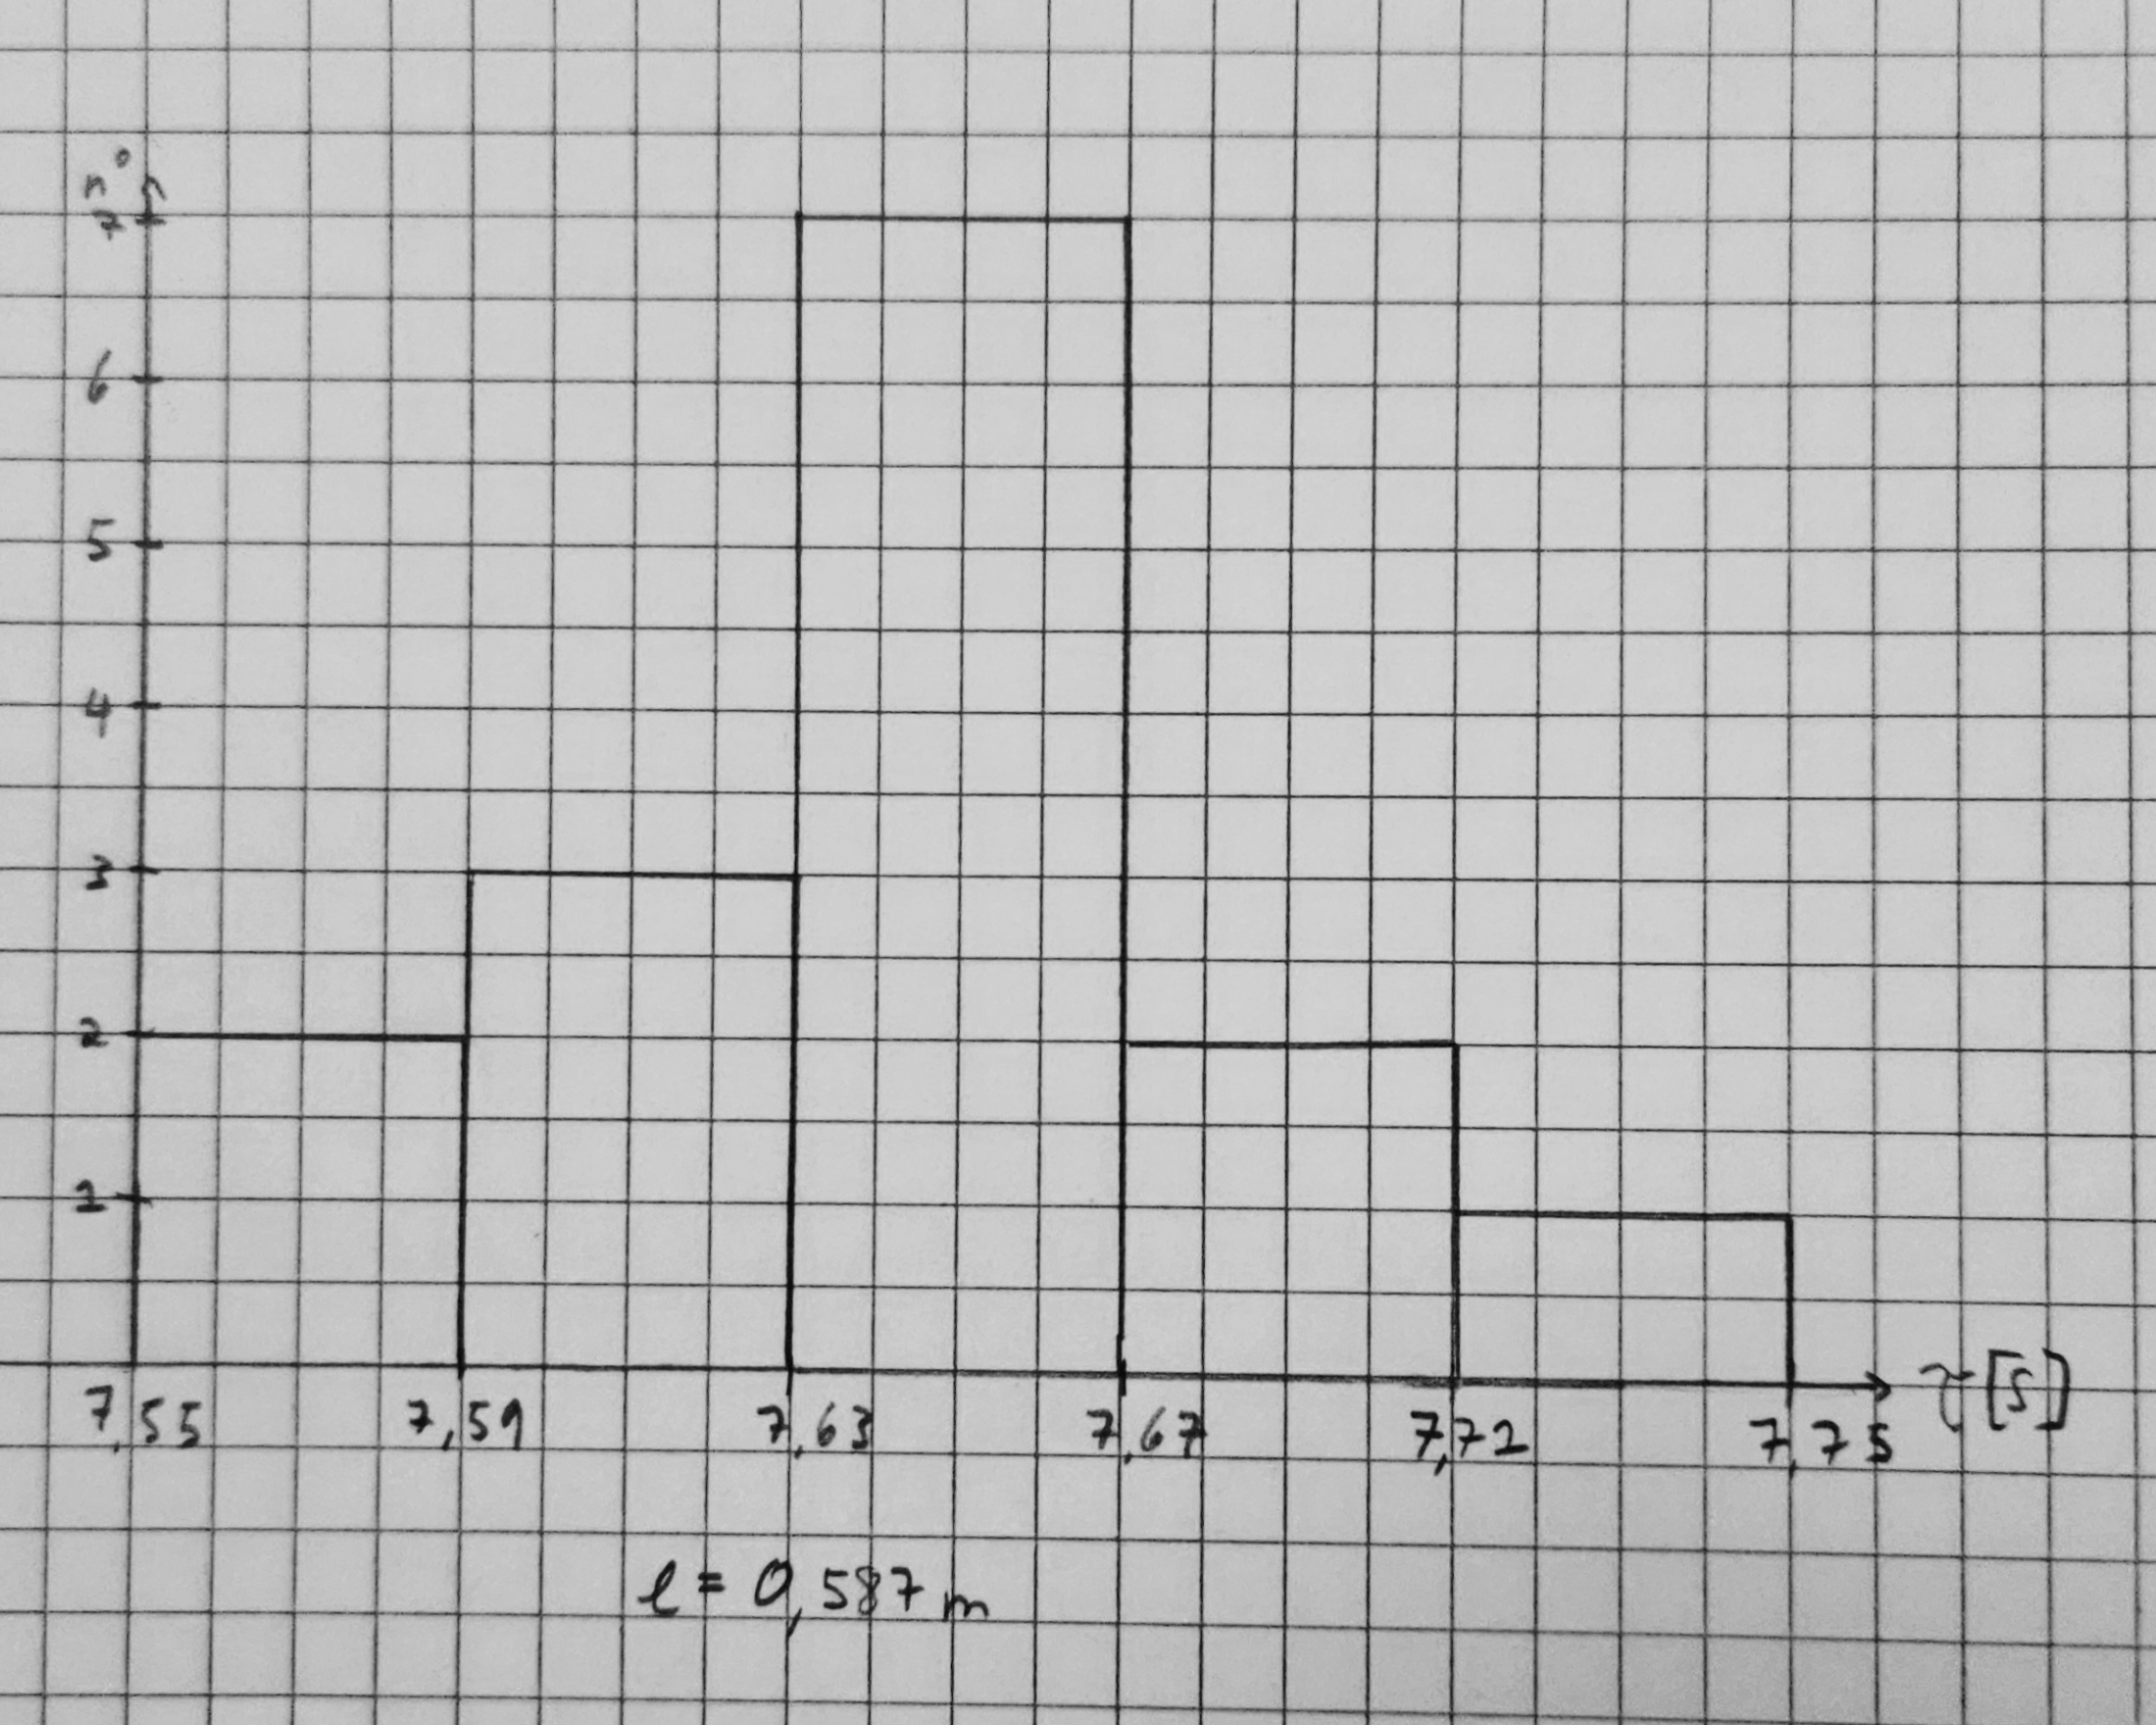
\includegraphics[width=\textwidth]{fotopendolo/lunghezza_0587.jpg}
      \caption{Misure con $l=0.587m$}
    \end{minipage}
  \end{figure}

\begin{figure}[!h]
    \centering
    \begin{minipage}[b]{0.4\textwidth}
      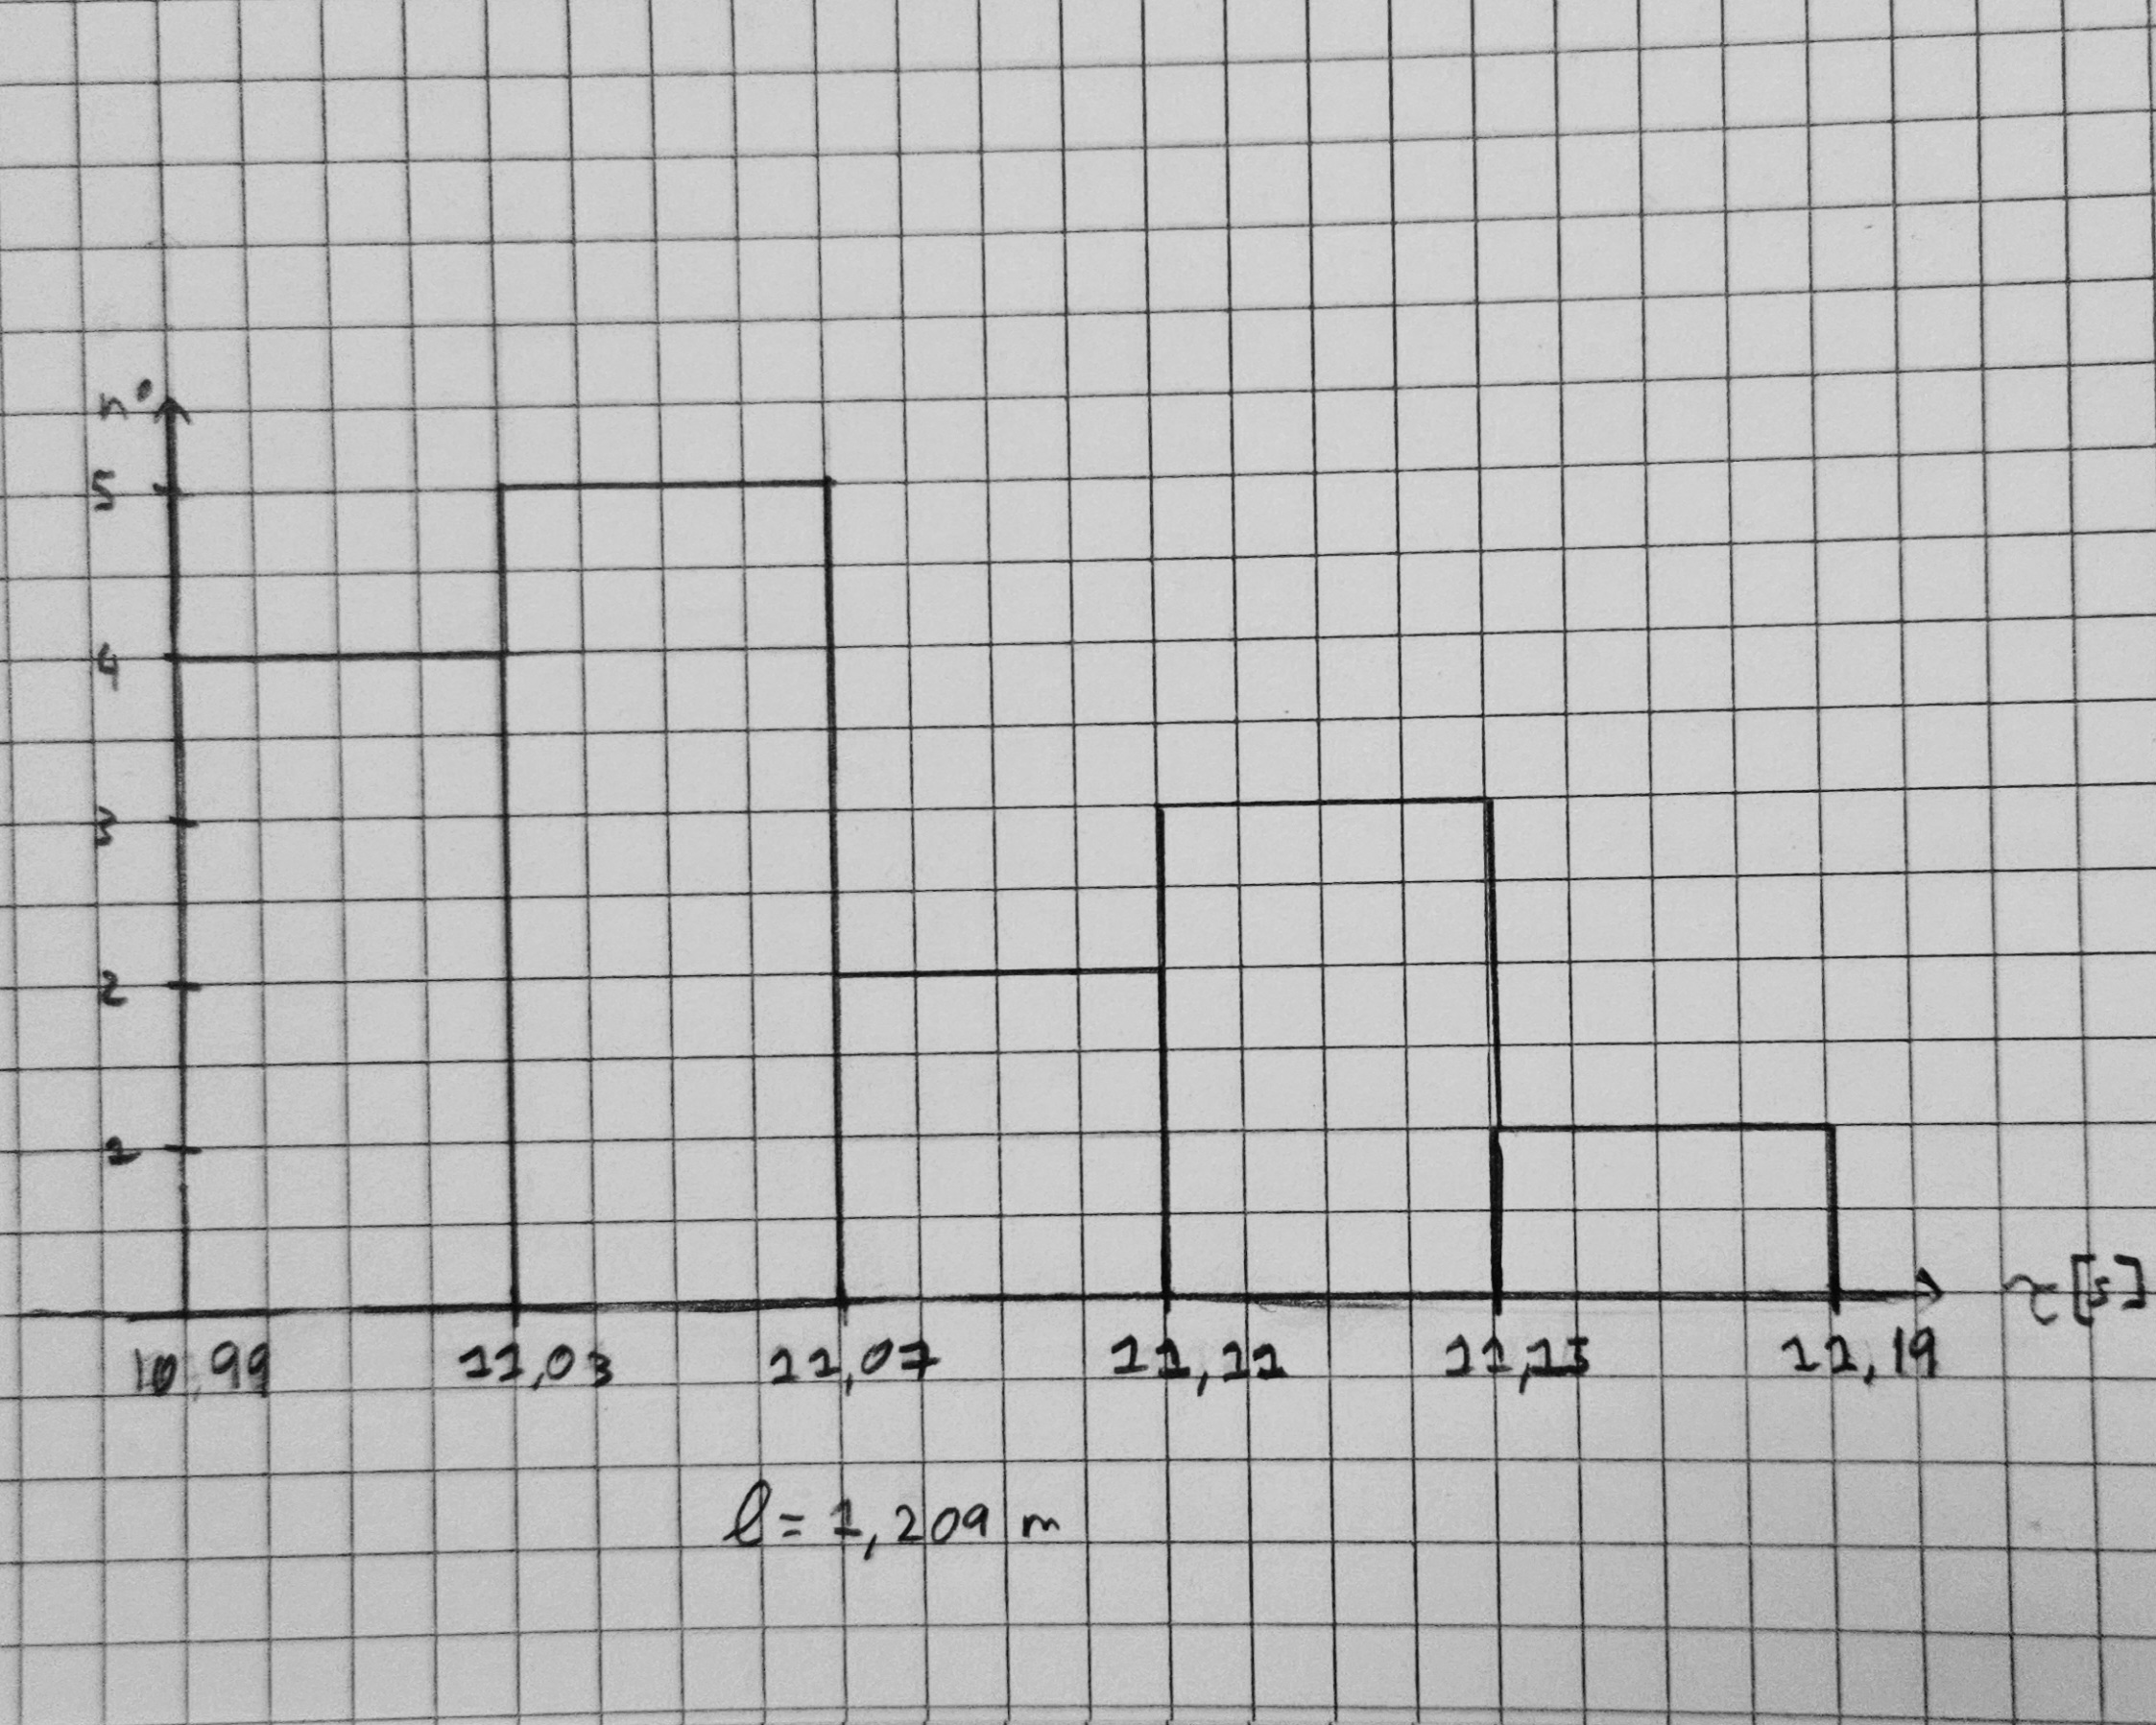
\includegraphics[width=\textwidth]{fotopendolo/lunghezza_1209.jpg}
      \caption{Misure con $l=1.209m$}
    \end{minipage}
    \hfill
    \begin{minipage}[b]{0.4\textwidth}
      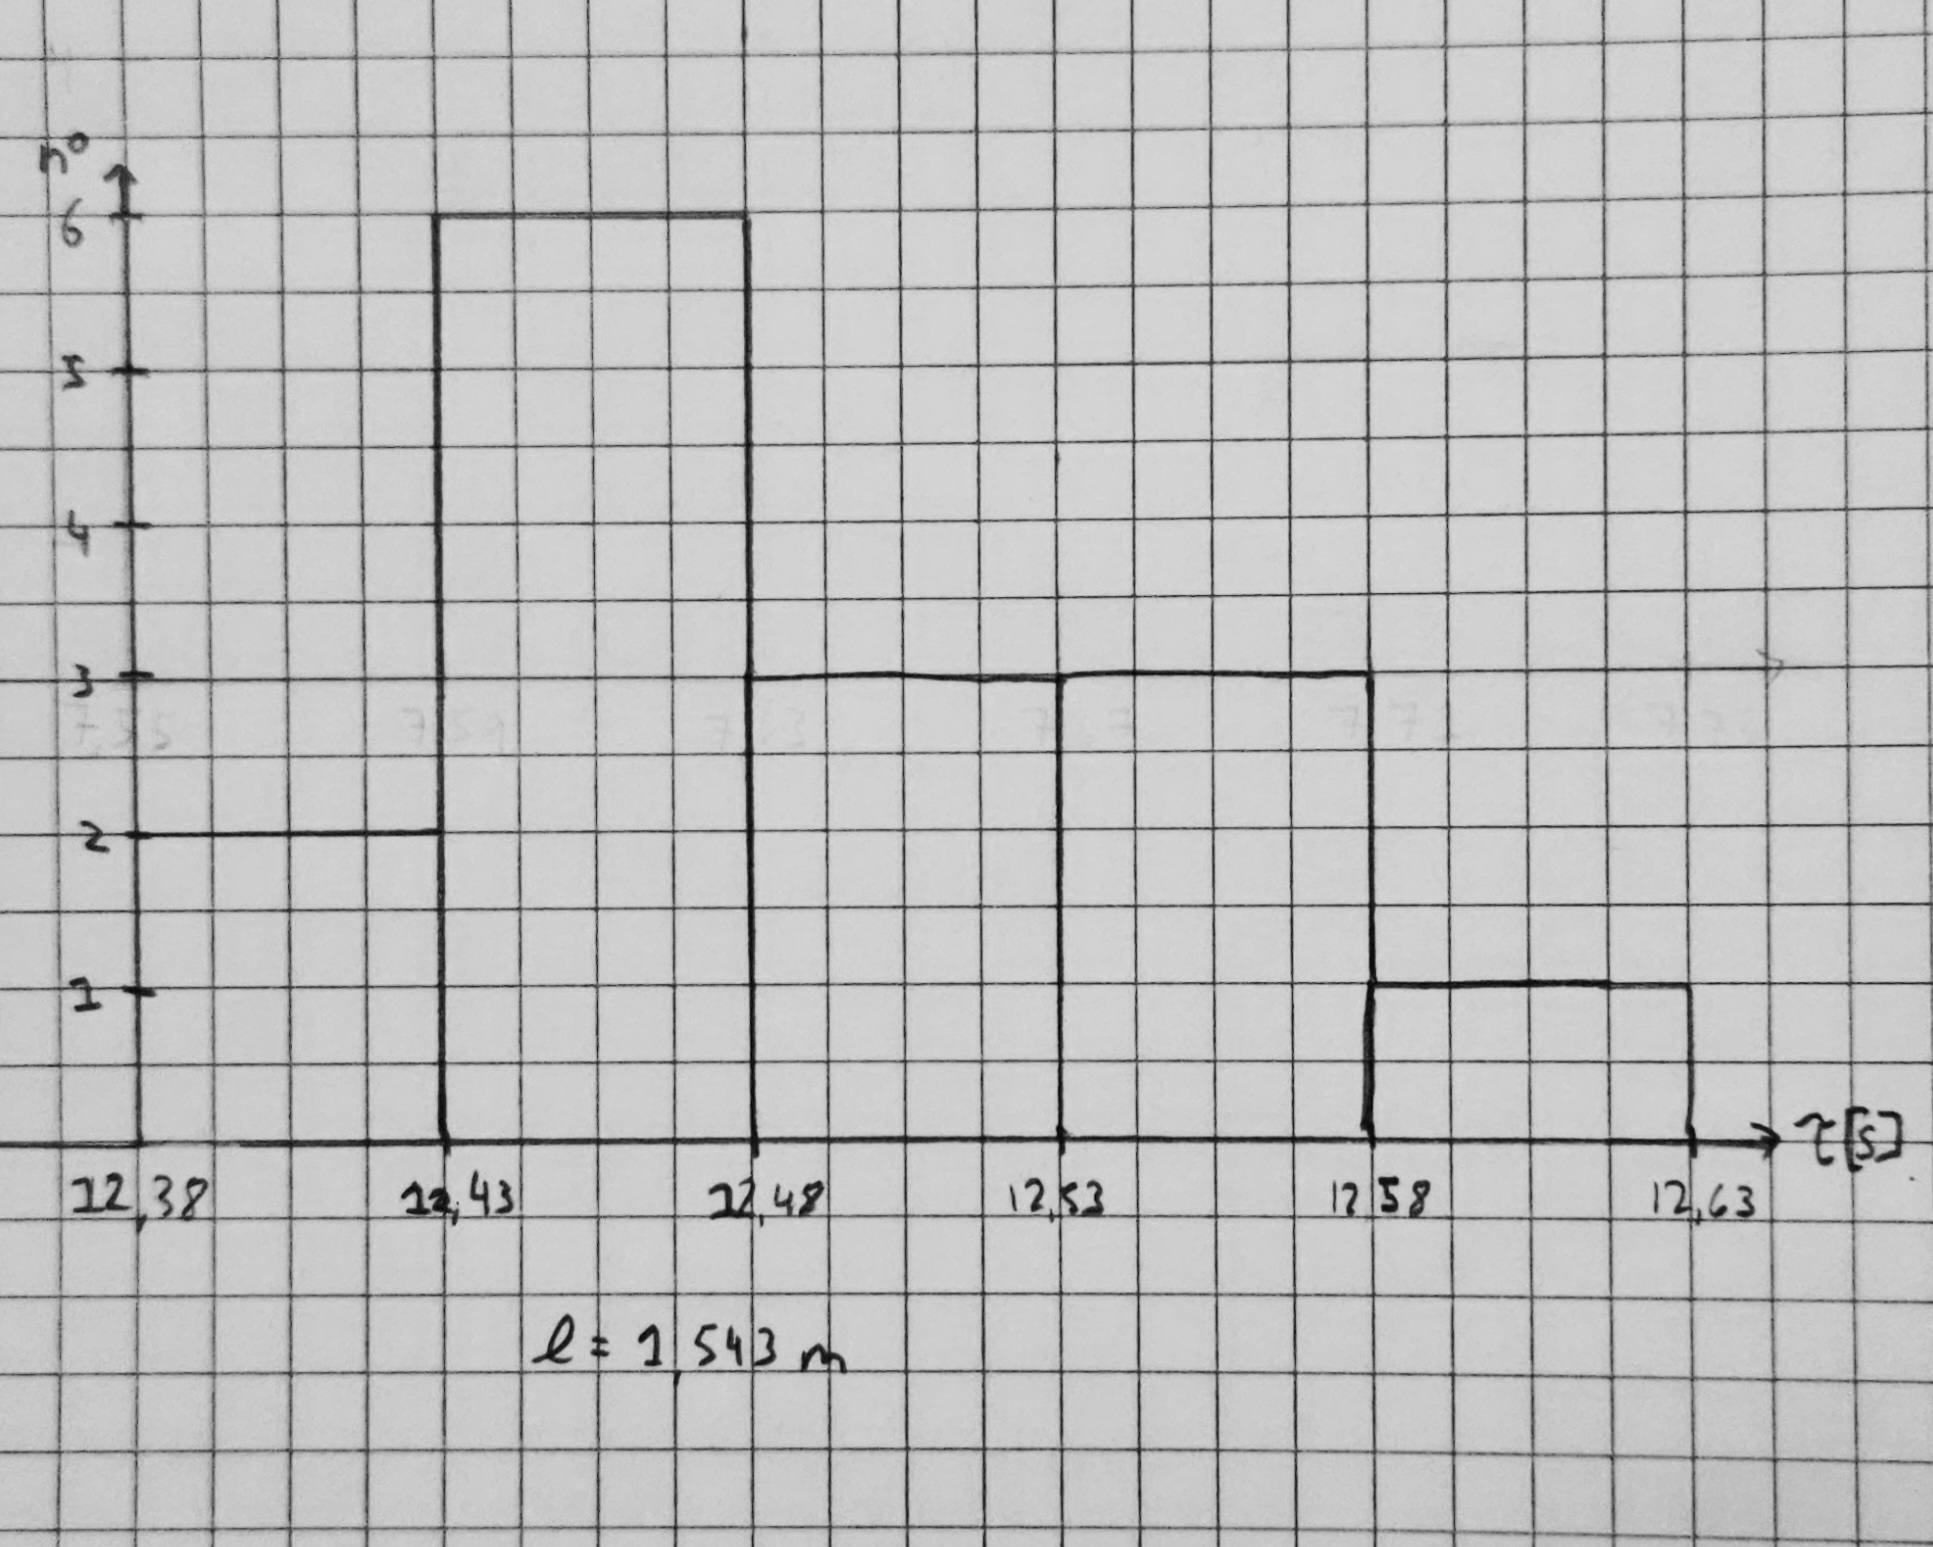
\includegraphics[width=\textwidth]{fotopendolo/lunghezza_1543.jpg}
      \caption{Misure con $l=1.543m$}
    \end{minipage}
  \end{figure}

\begin{figure}[!h]
    \centering
    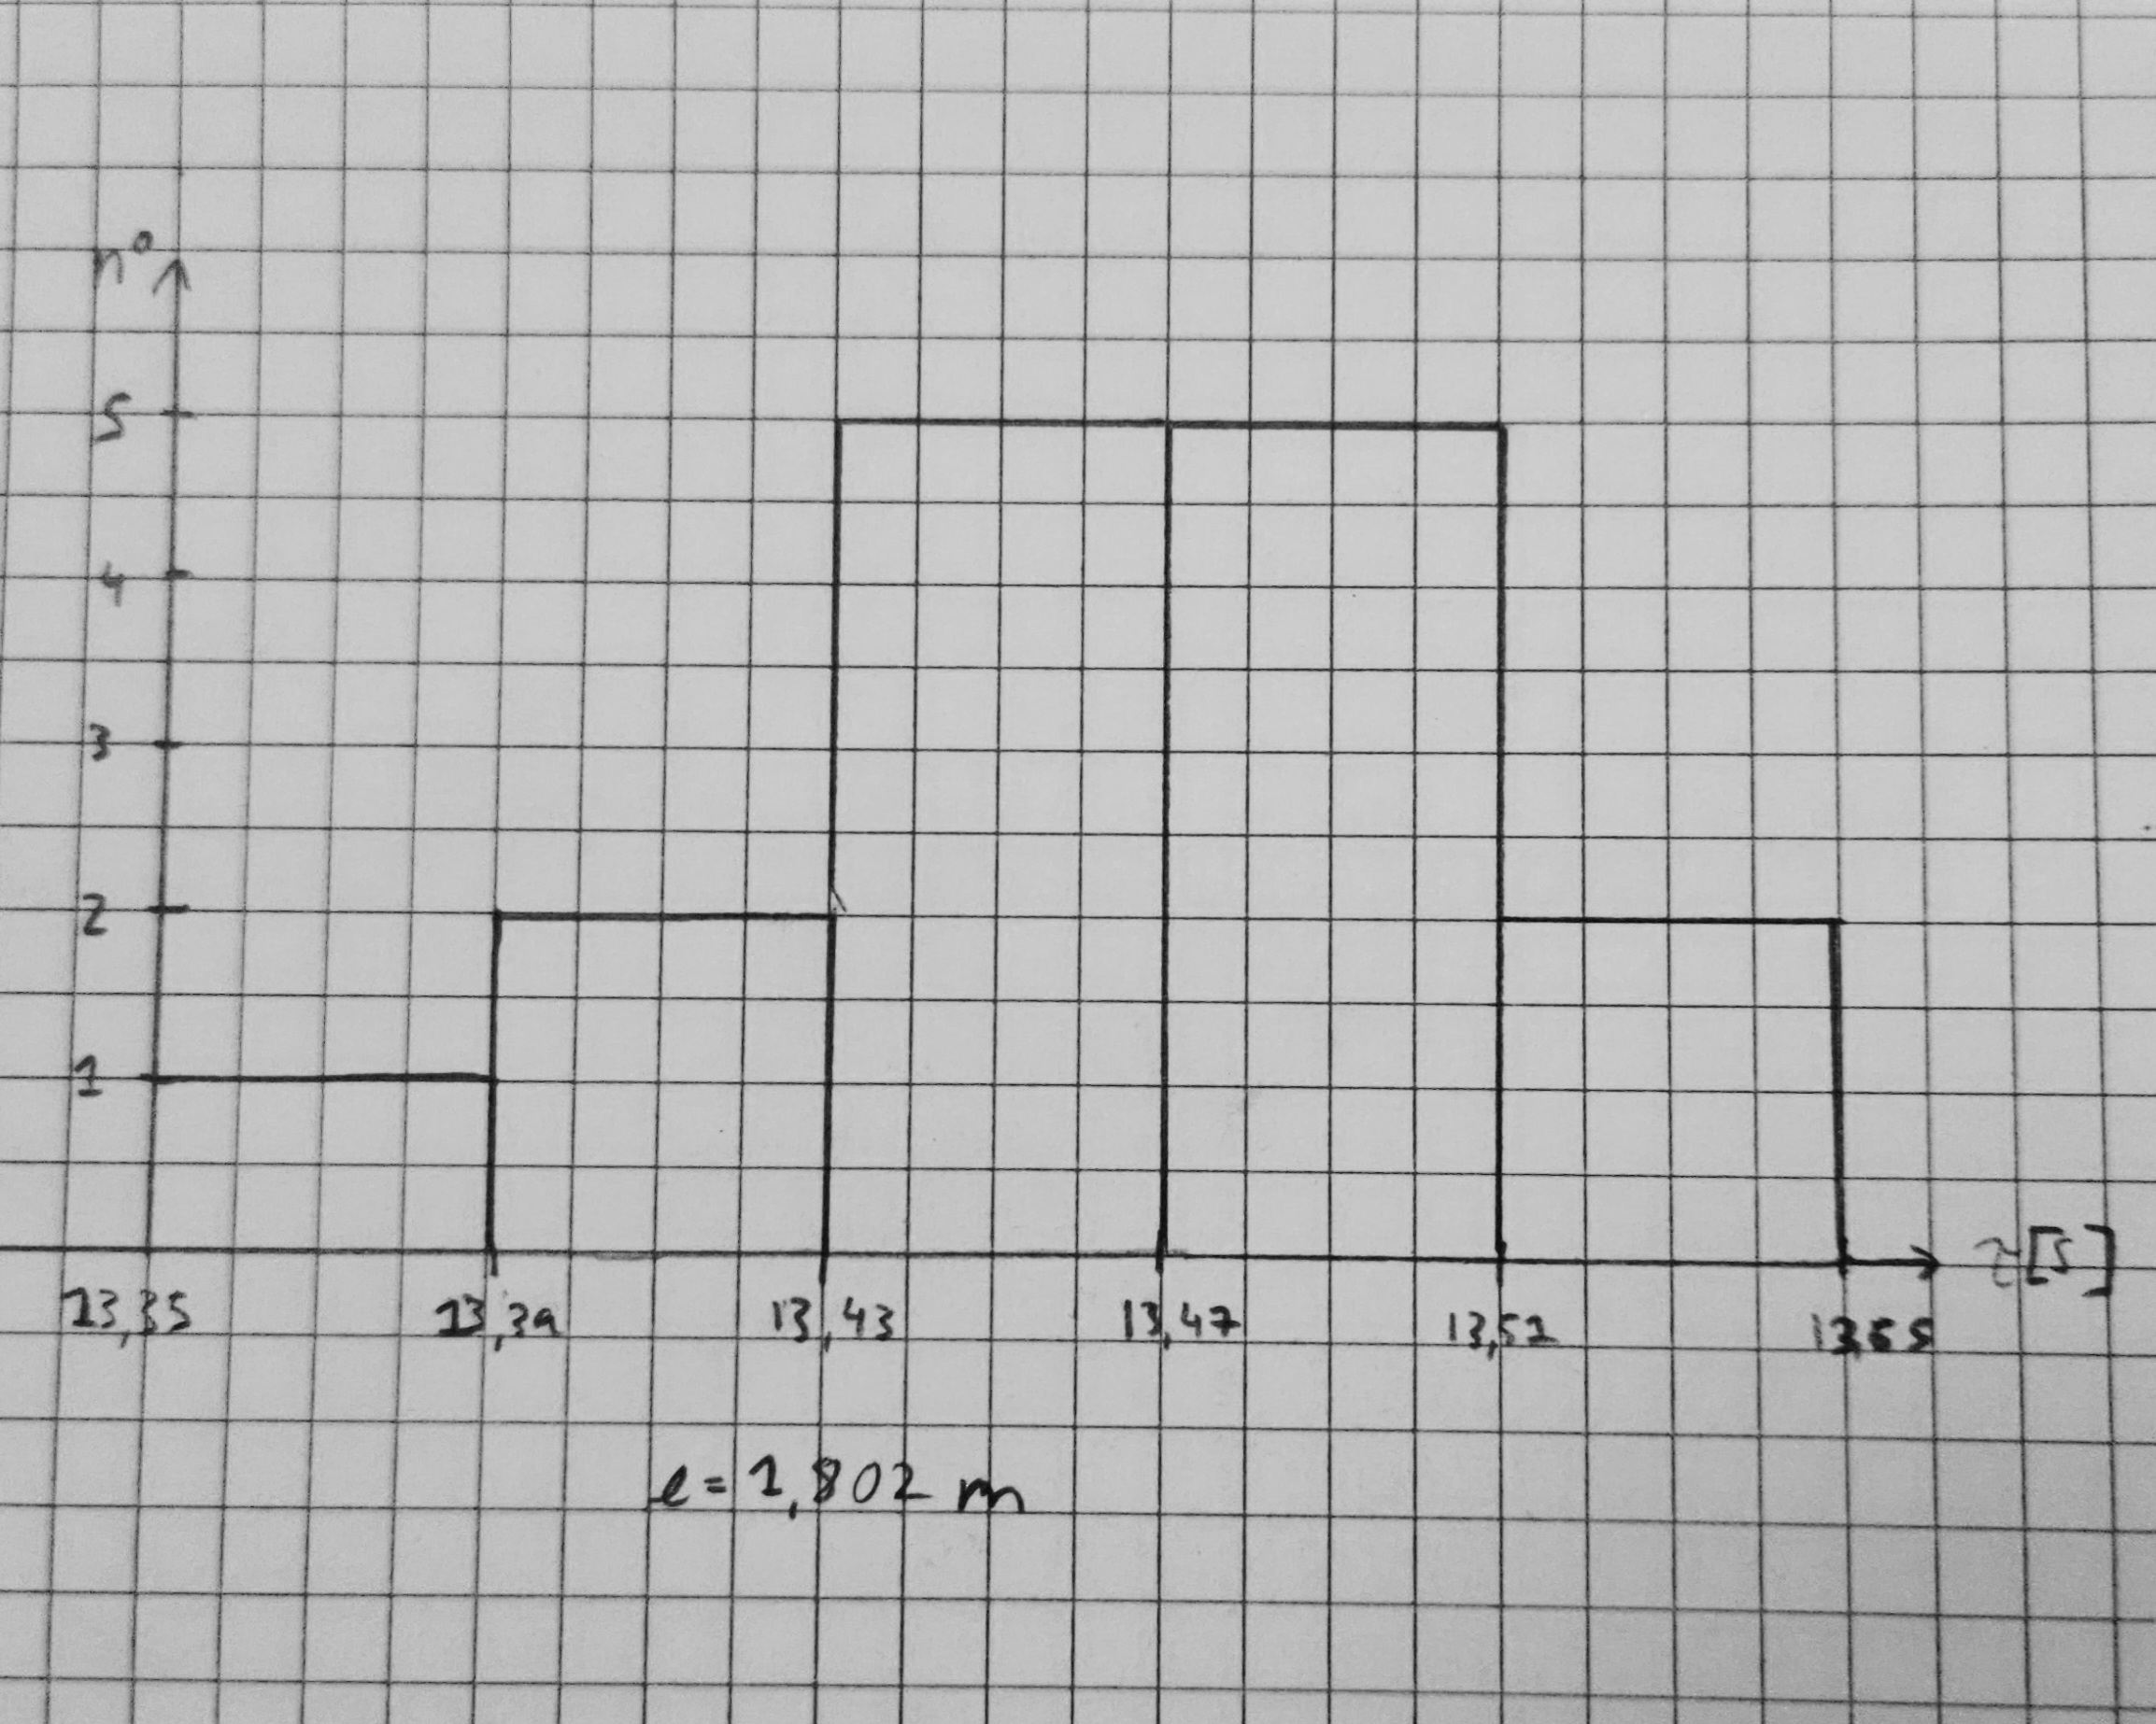
\includegraphics[width=0.4\textwidth]{fotopendolo/lunghezza_1802.jpg}
    \caption{Misure con $l=1.802m$}
\end{figure}
\subsubsection{Istogrammi $l=0.991m$}
\begin{figure}[!h]
    \centering
    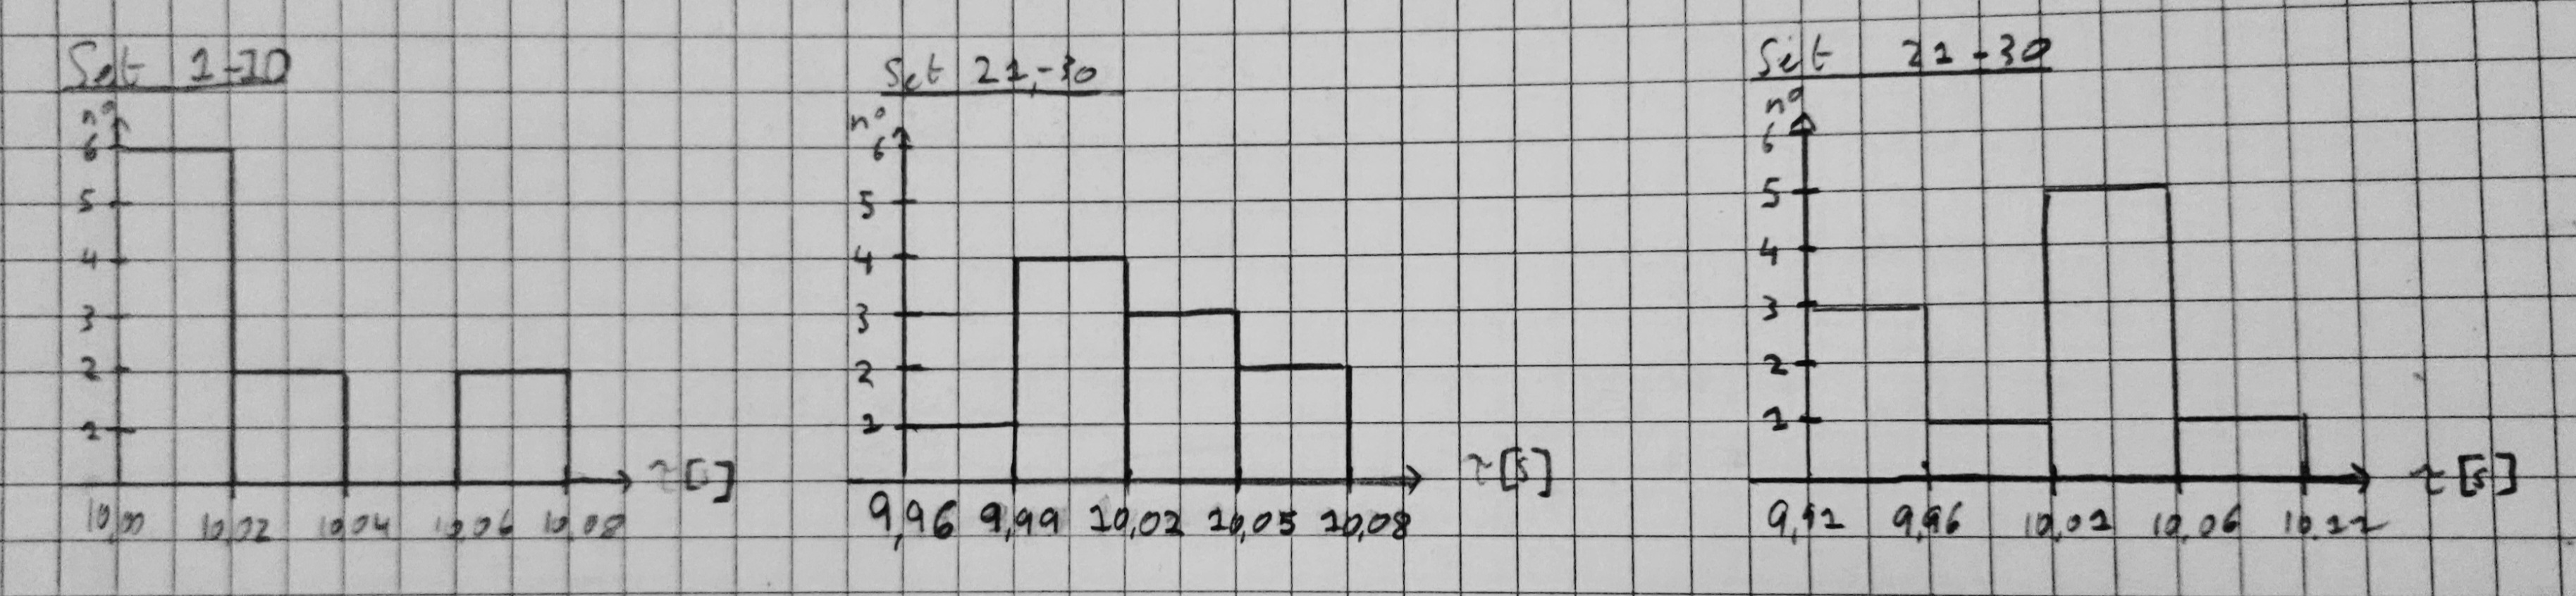
\includegraphics[width=\textwidth]{fotopendolo/set1-30.jpg}
    \caption{Set di misure 1-30}
\end{figure}
\begin{figure}[!h]
    \centering
    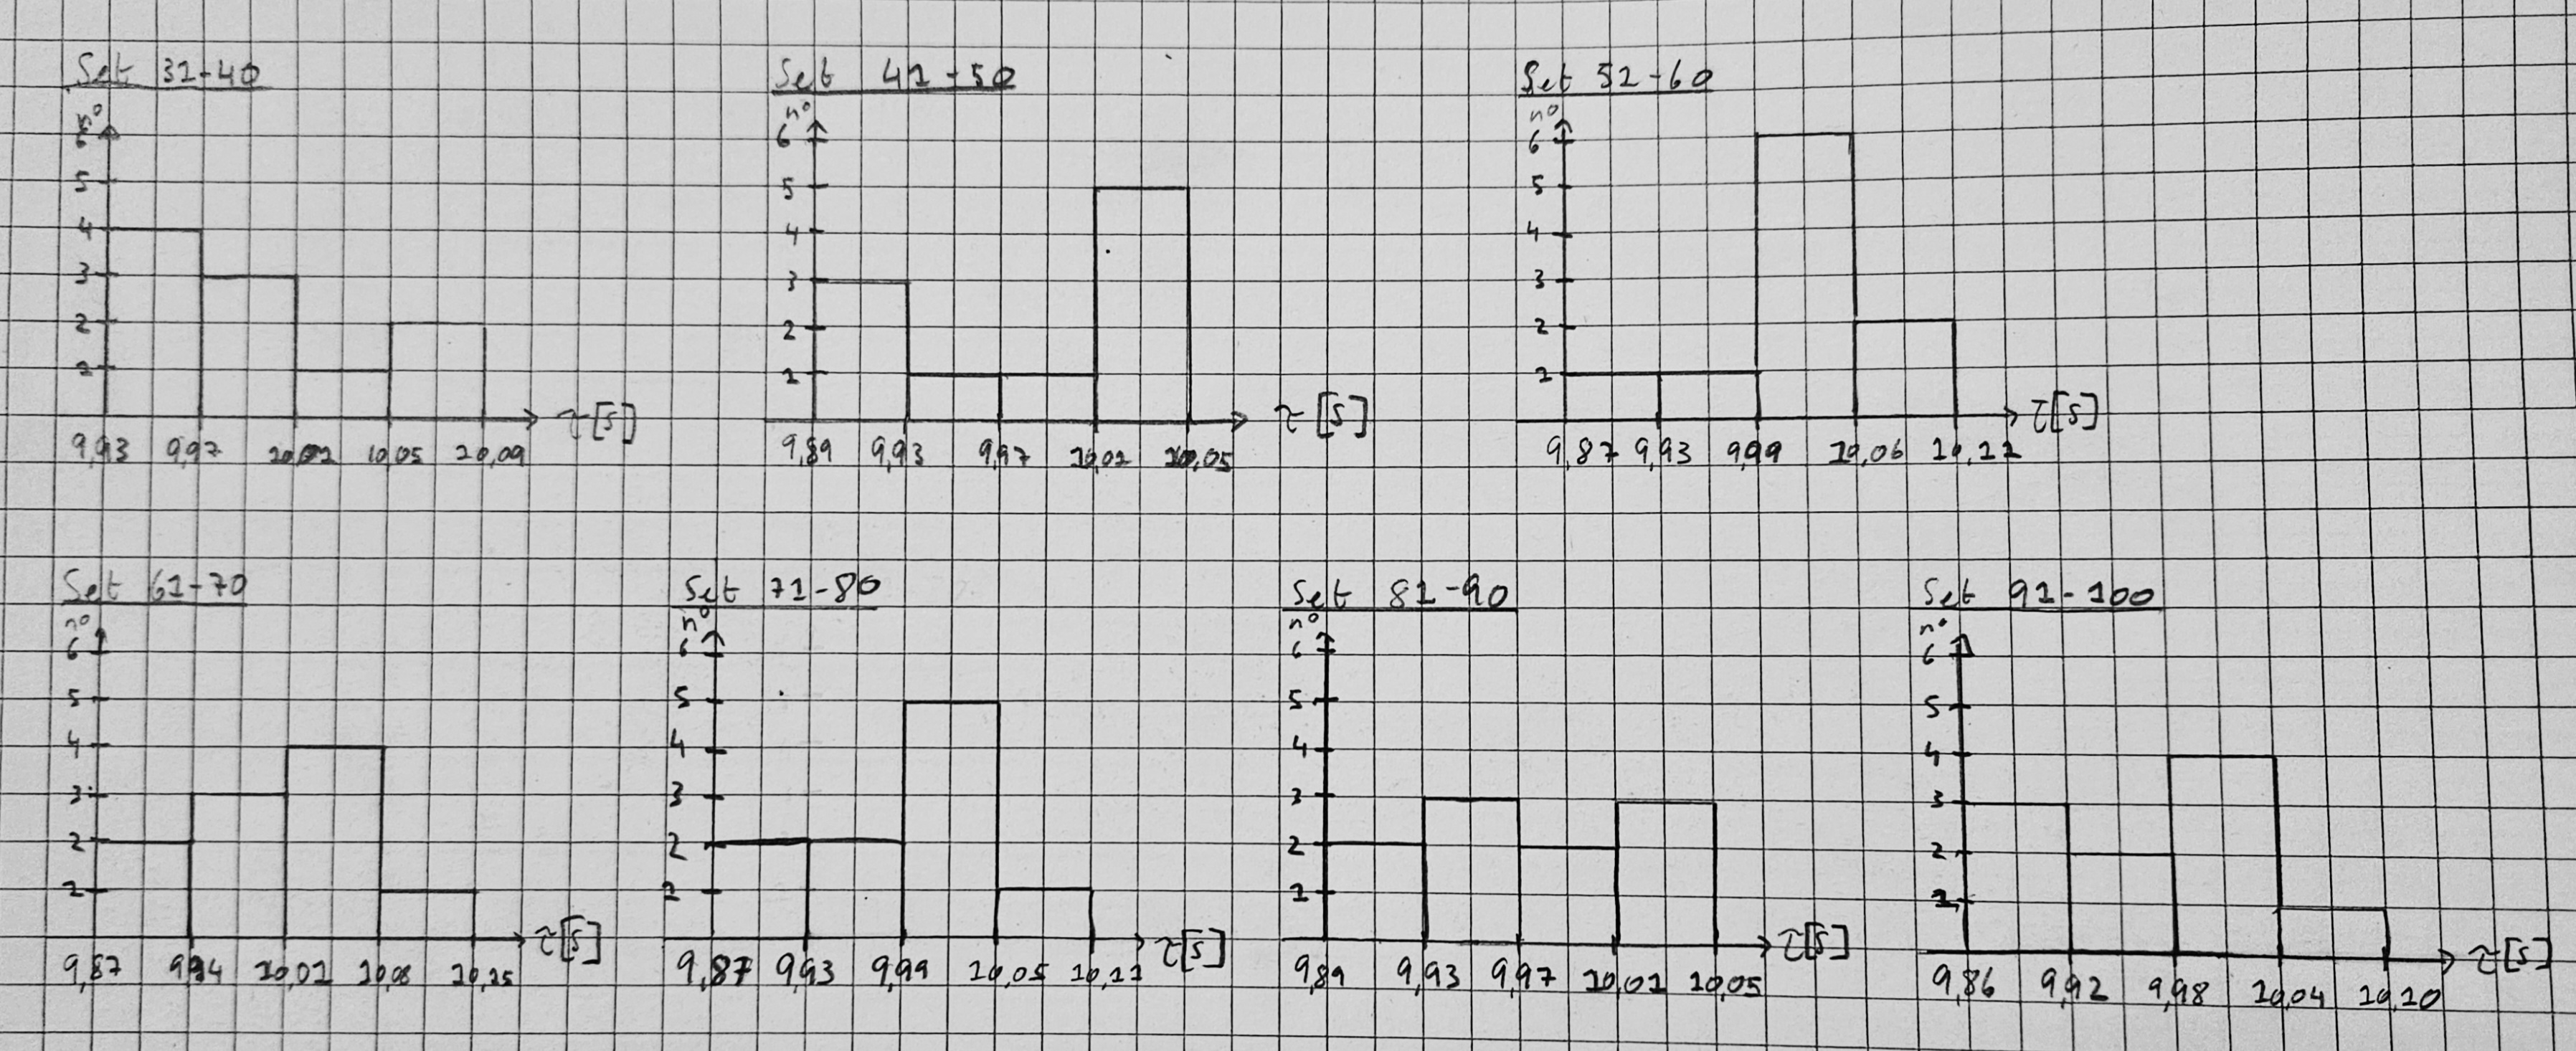
\includegraphics[width=\textwidth]{fotopendolo/setresto.jpg}
    \caption{Set di misure 31-100}
\end{figure}
\begin{figure}[!h]
    \centering
    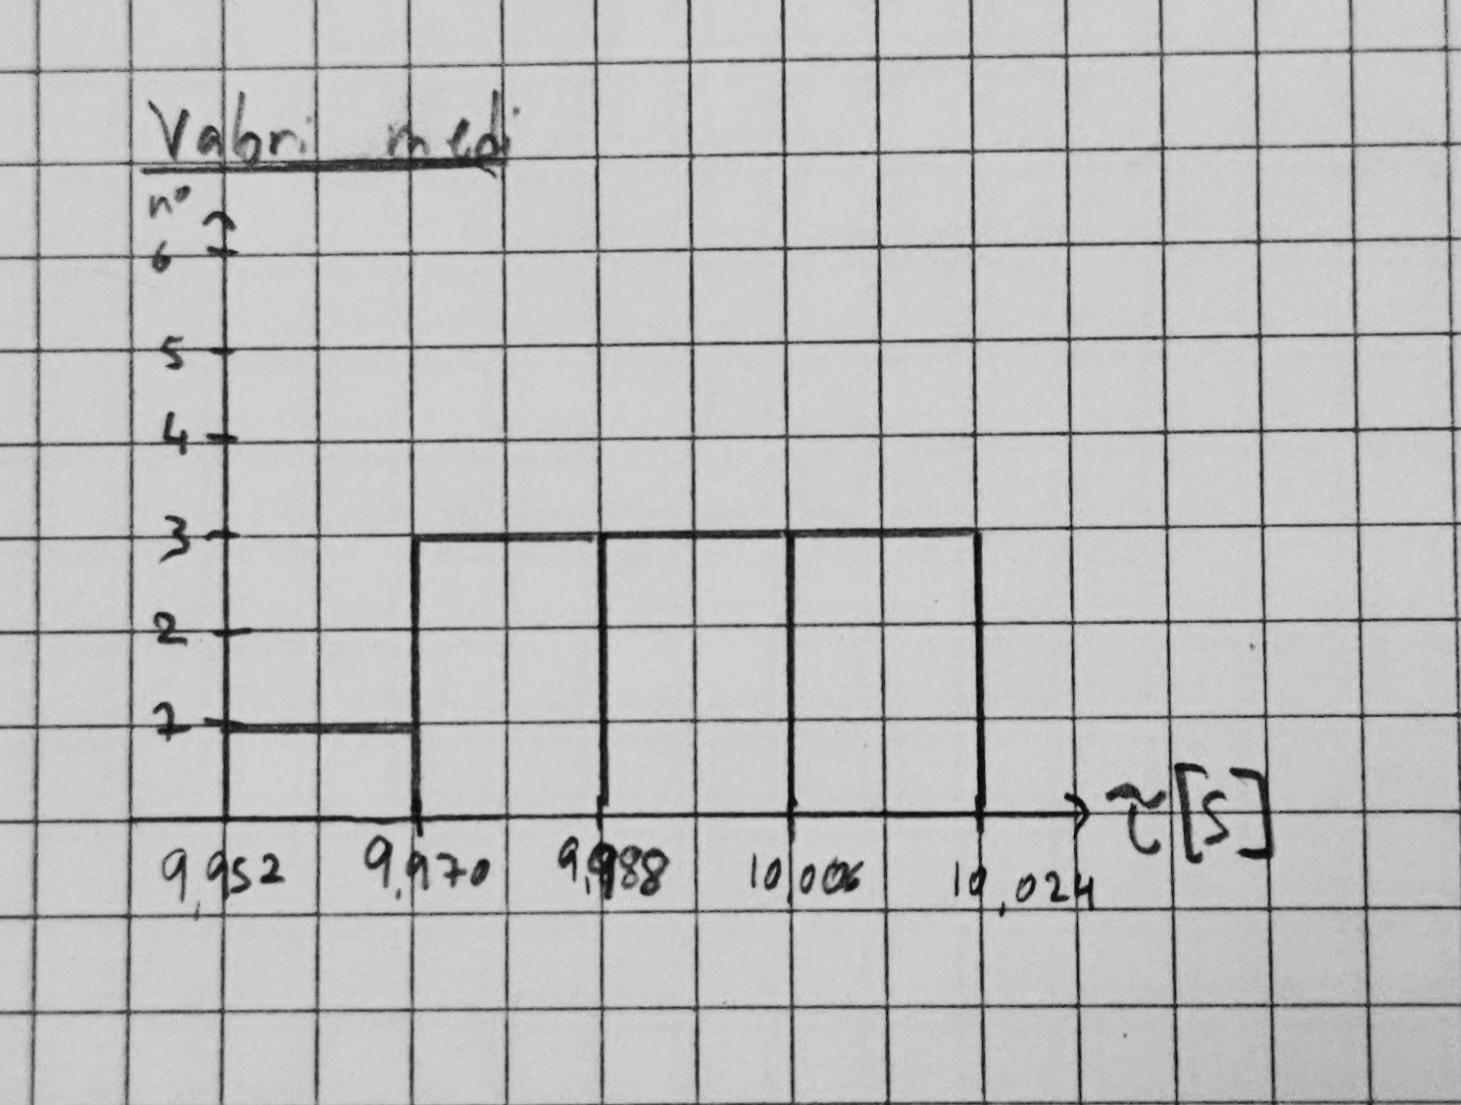
\includegraphics[width=\textwidth]{fotopendolo/setmedi.jpg}
    \caption{Istogramma della media dei 10 set}
\end{figure}
\begin{figure}[!h]
    \centering
    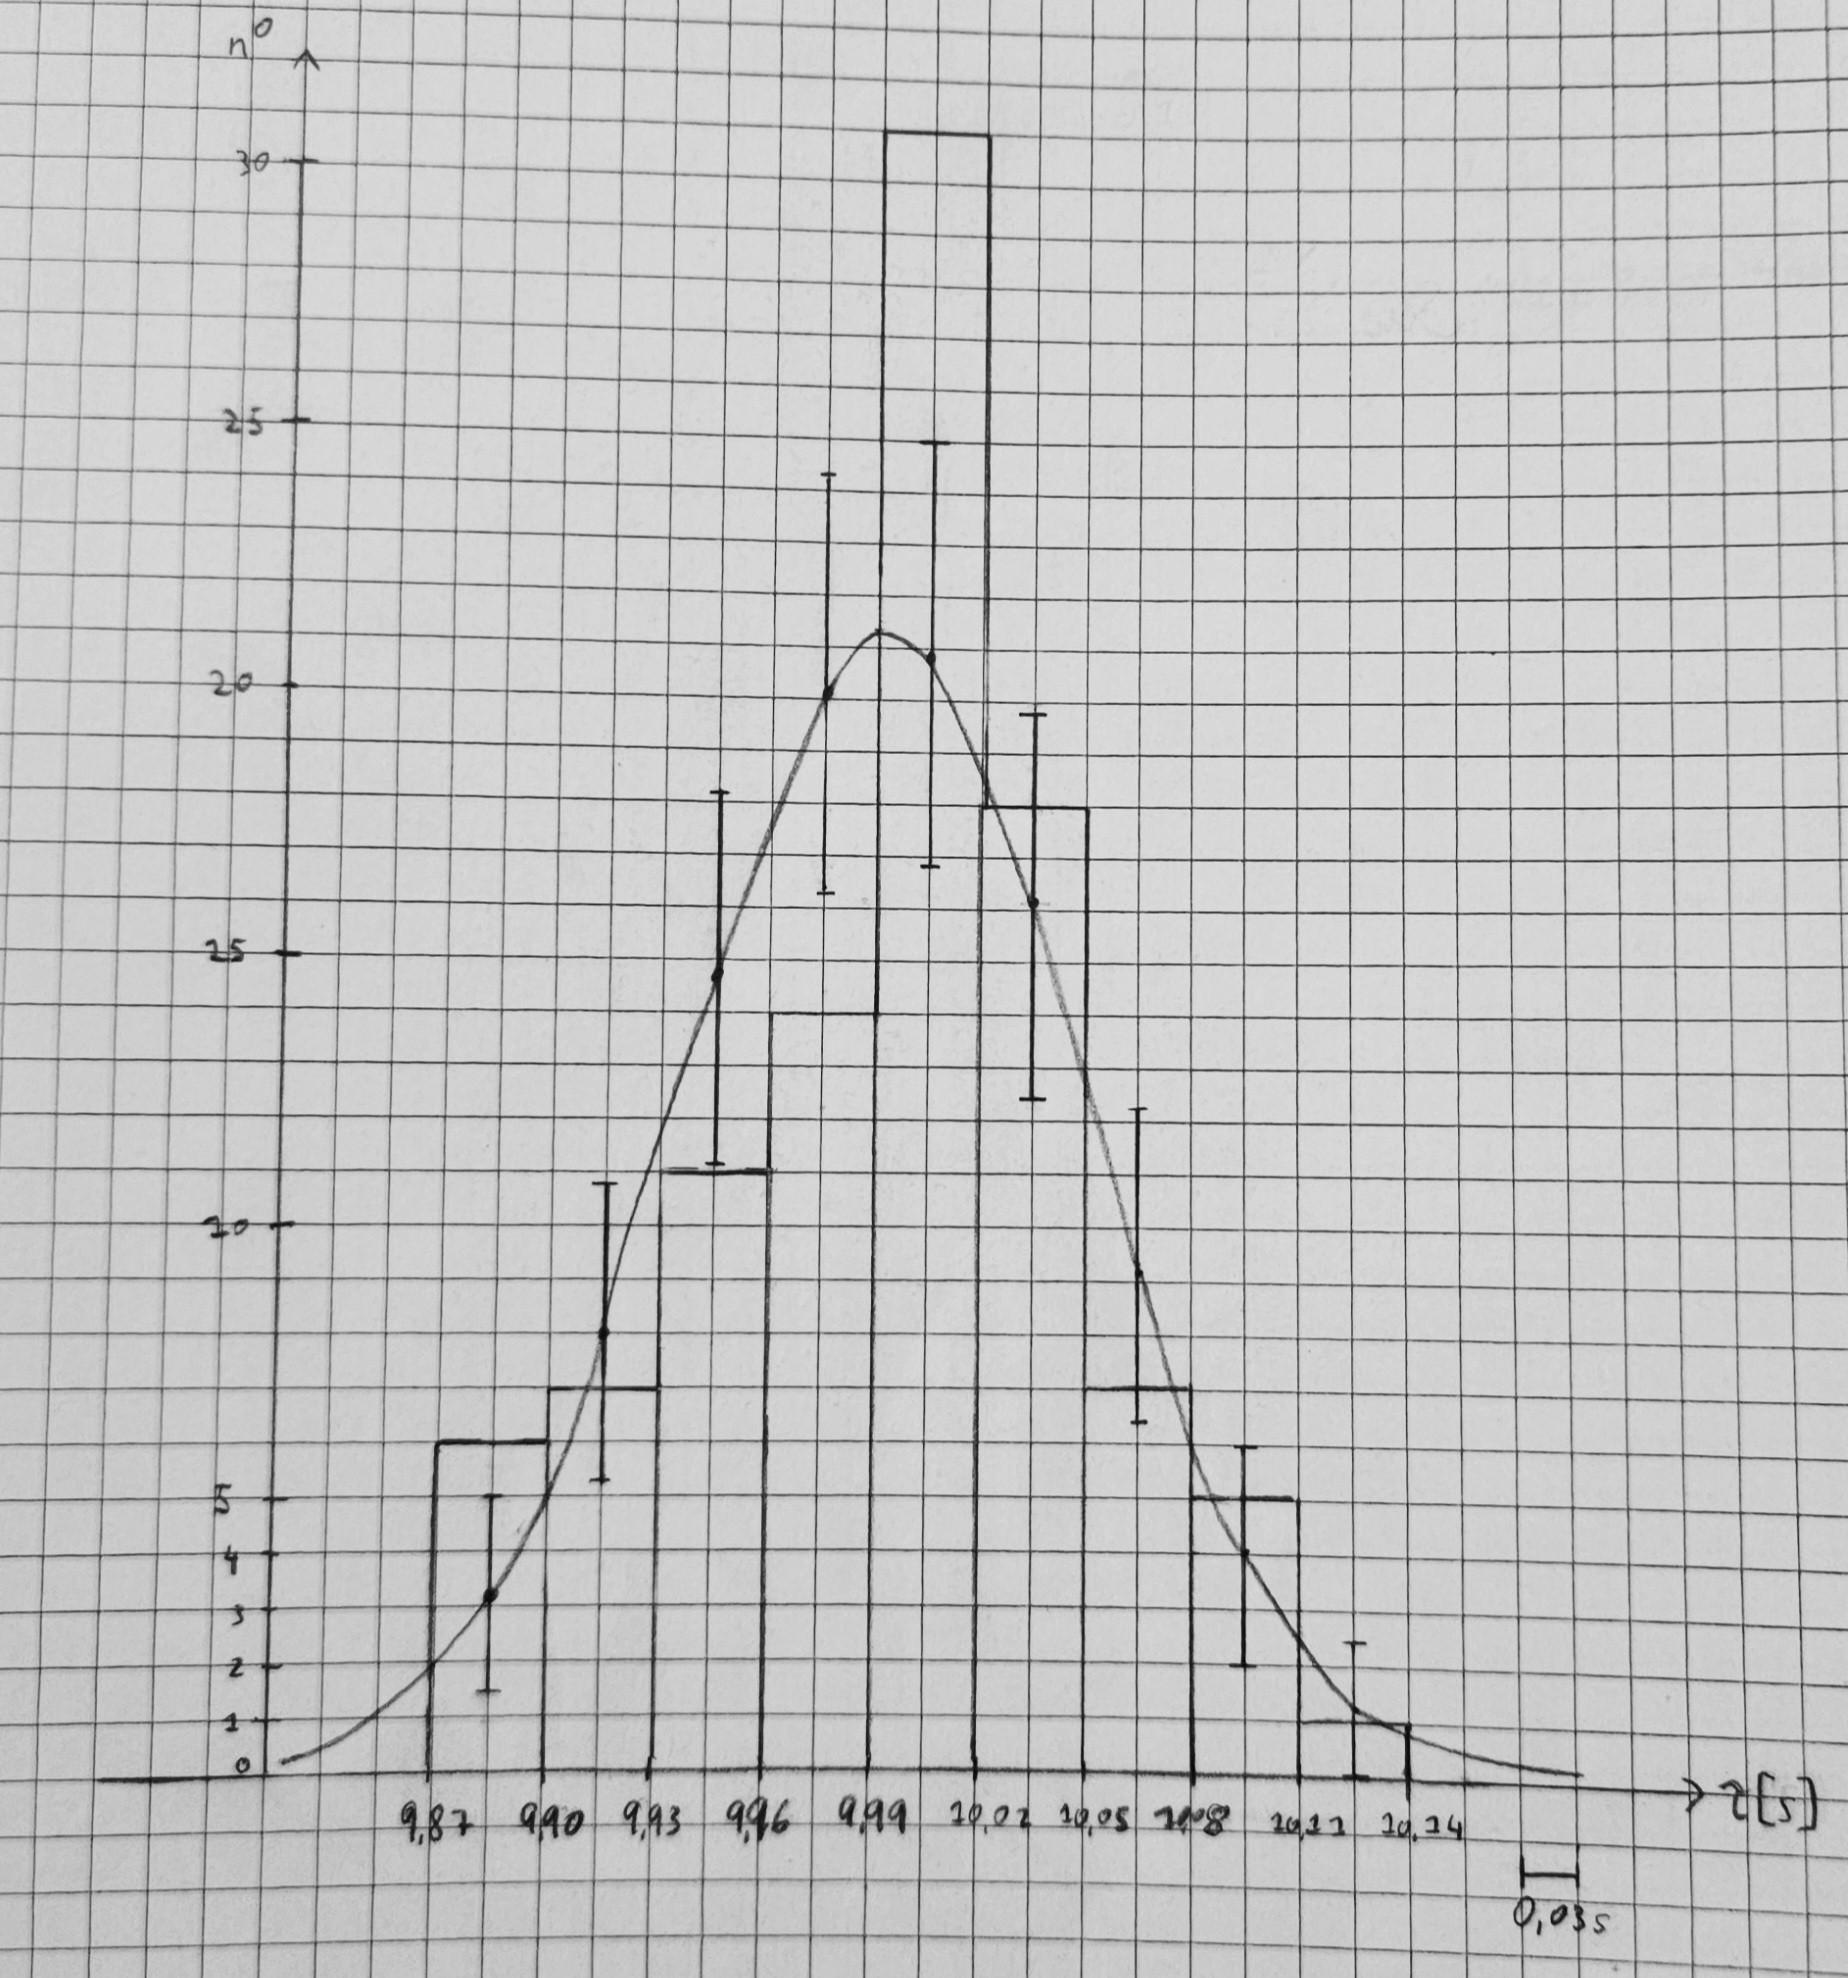
\includegraphics[width=\textwidth]{fotopendolo/gaussiana.jpg}
    \caption{Istogramma-Gaussiana per $l=0.991m$}
\end{figure}
\FloatBarrier

\newpage
\subsection{Grafici}
\subsubsection{Grafici di $T$ vs $l^{\alpha}$}
\begin{figure}[!h]
    \centering
    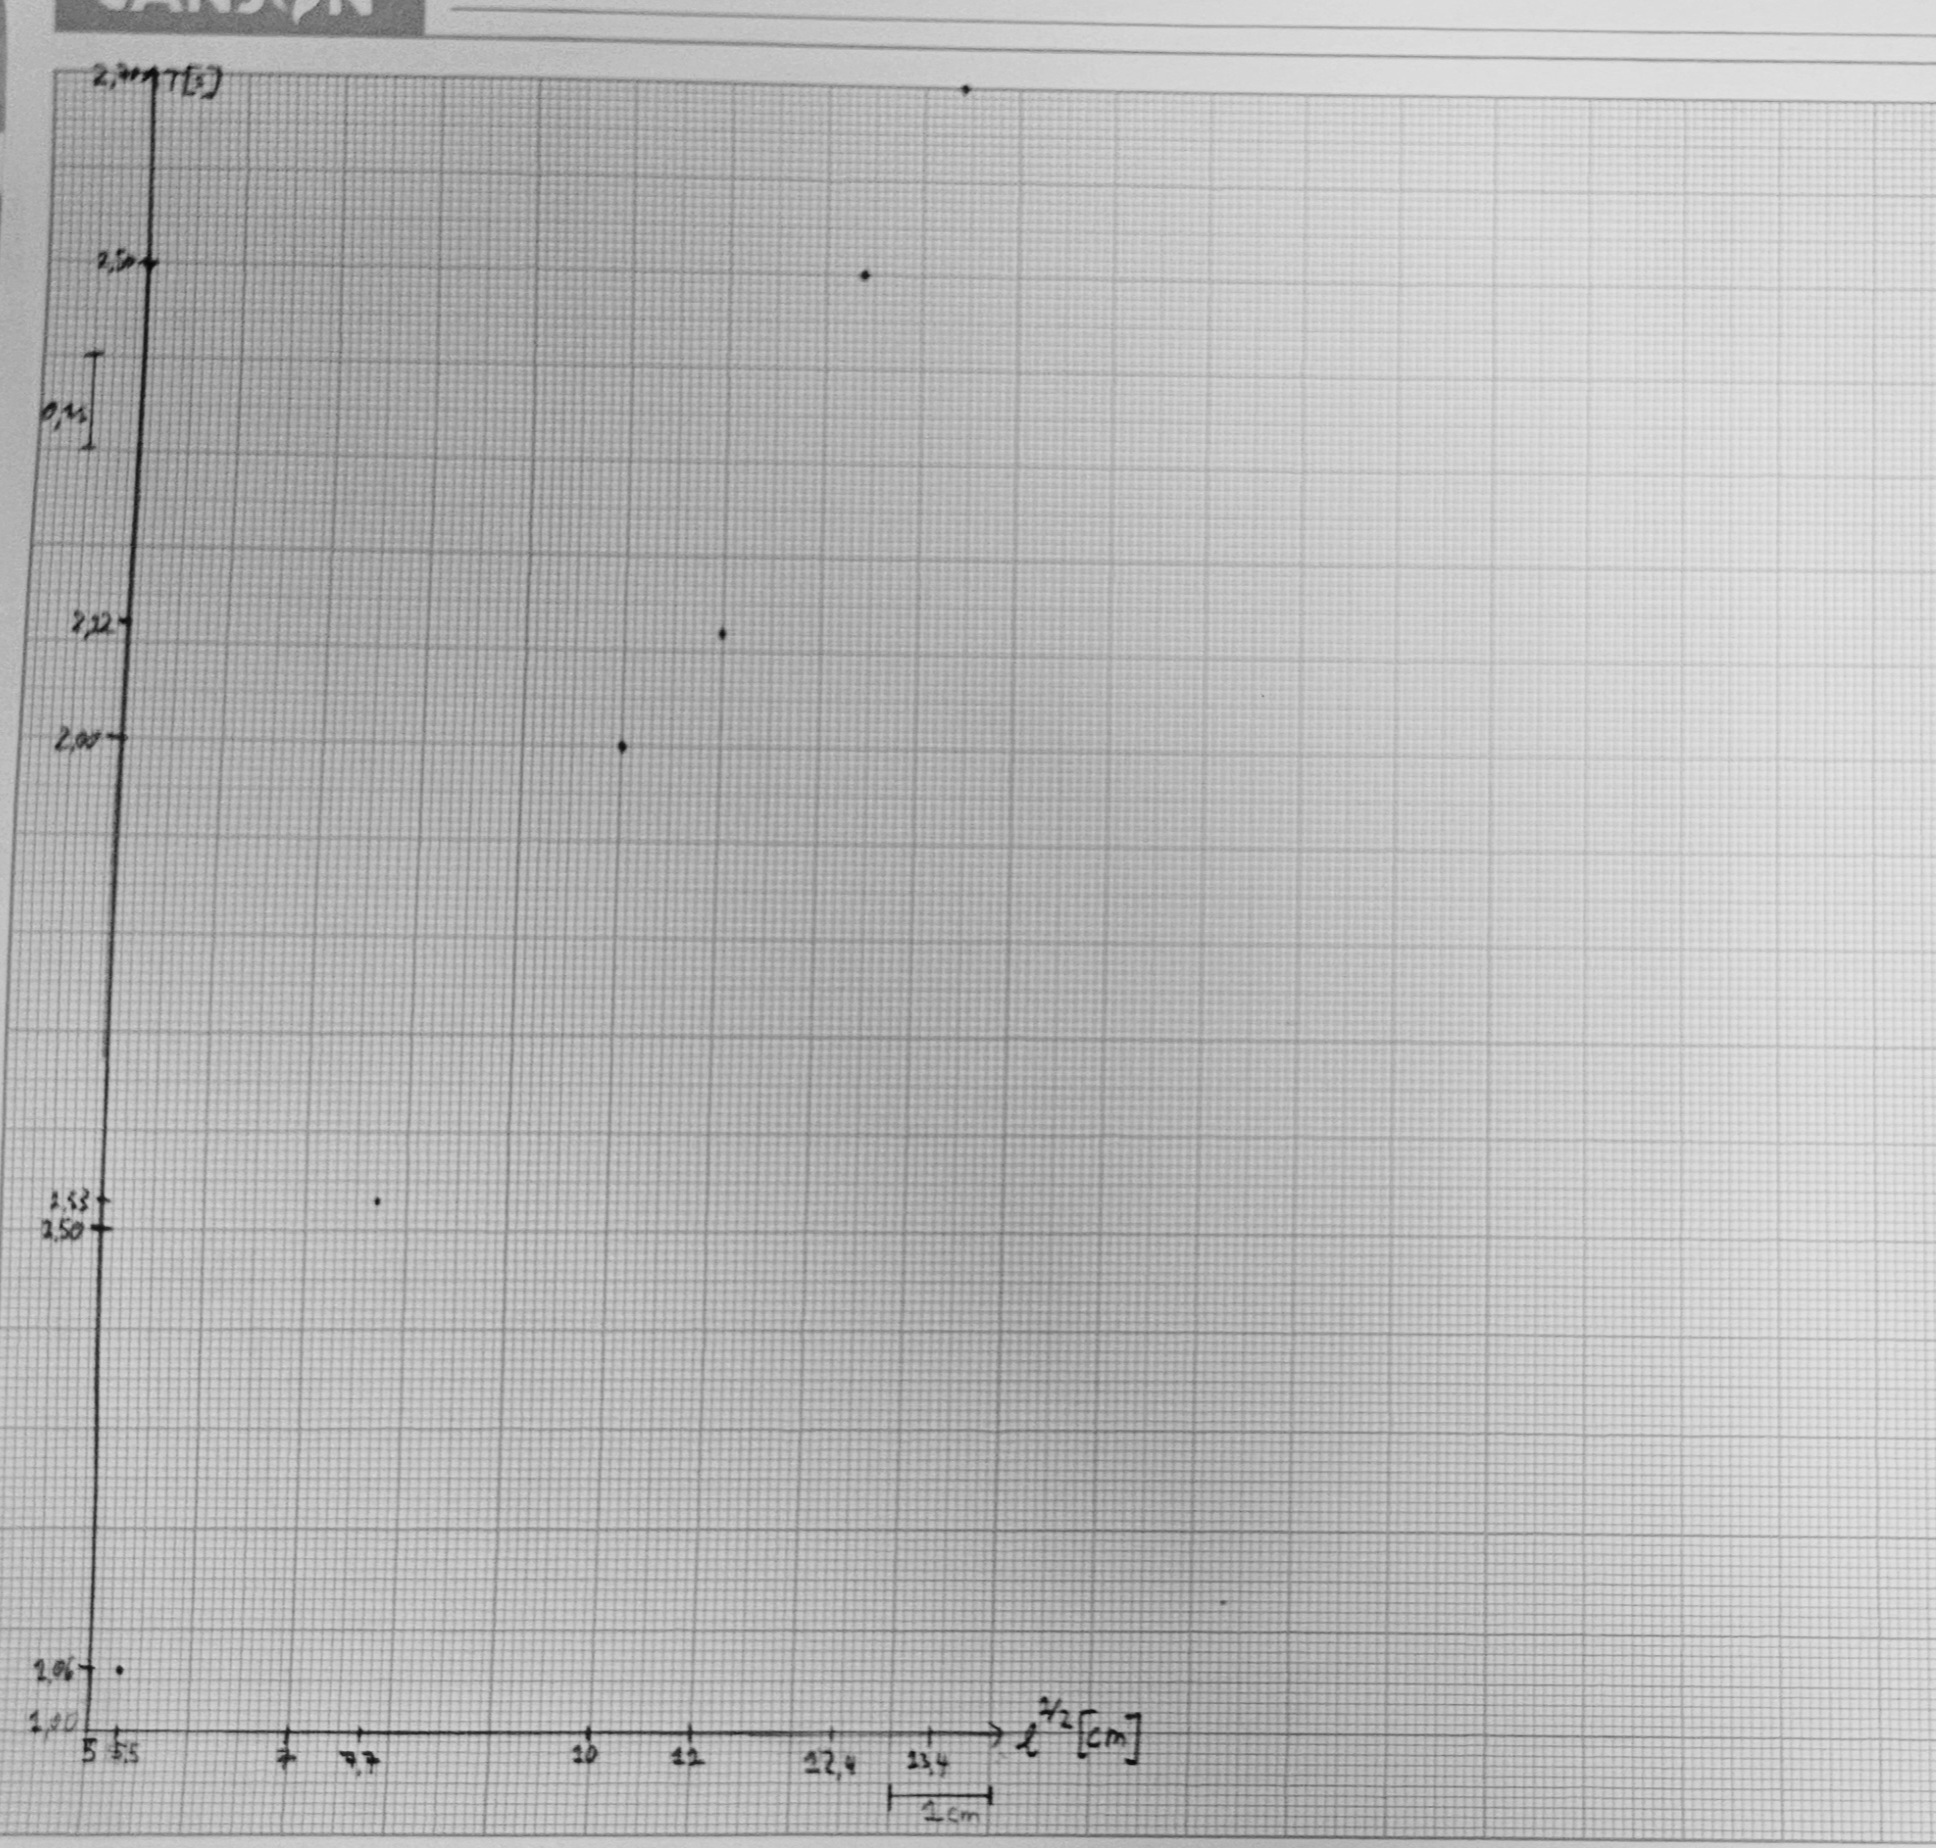
\includegraphics[width=0.75\textwidth]{fotopendolo/lunghezza12.jpg}
    \caption{Grafico $T$ vs $l^{1/2}$}
\end{figure}
\FloatBarrier
\begin{figure}[!h]
    \centering
    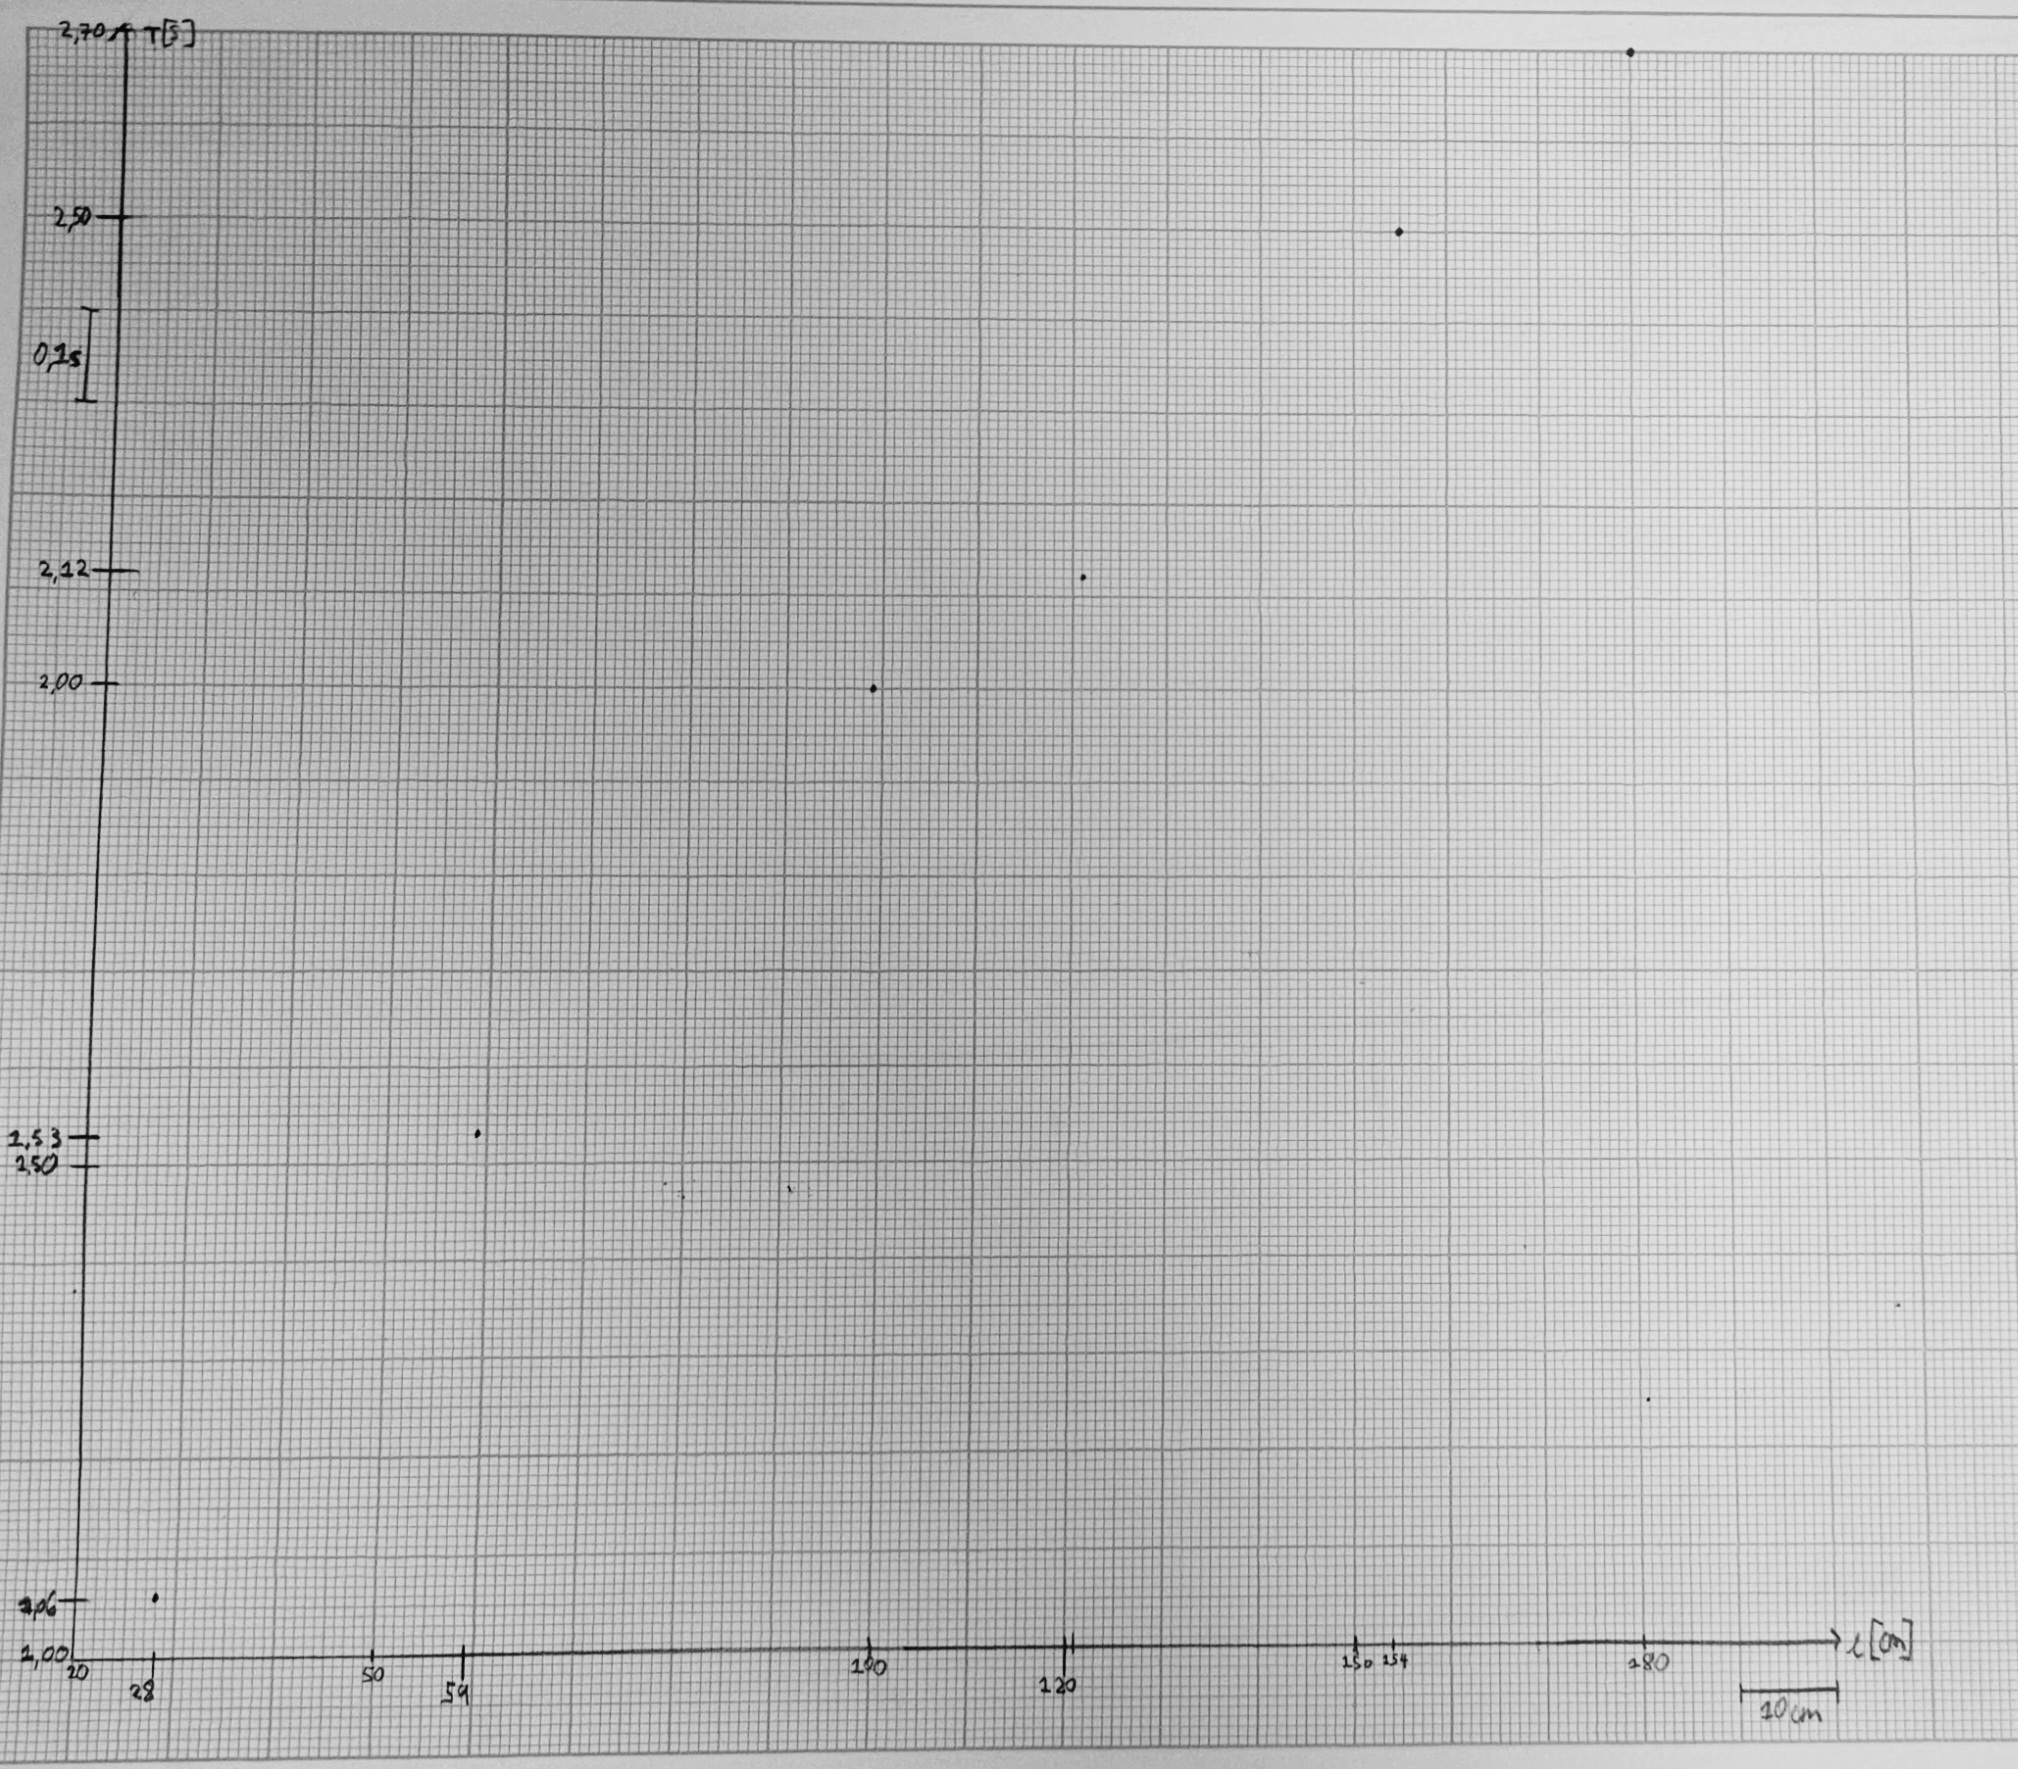
\includegraphics[width=0.75\textwidth]{fotopendolo/lunghezza11.jpg}
    \caption{Grafico $T$ vs $l$}
\end{figure}

\begin{figure}[!h]
    \centering
    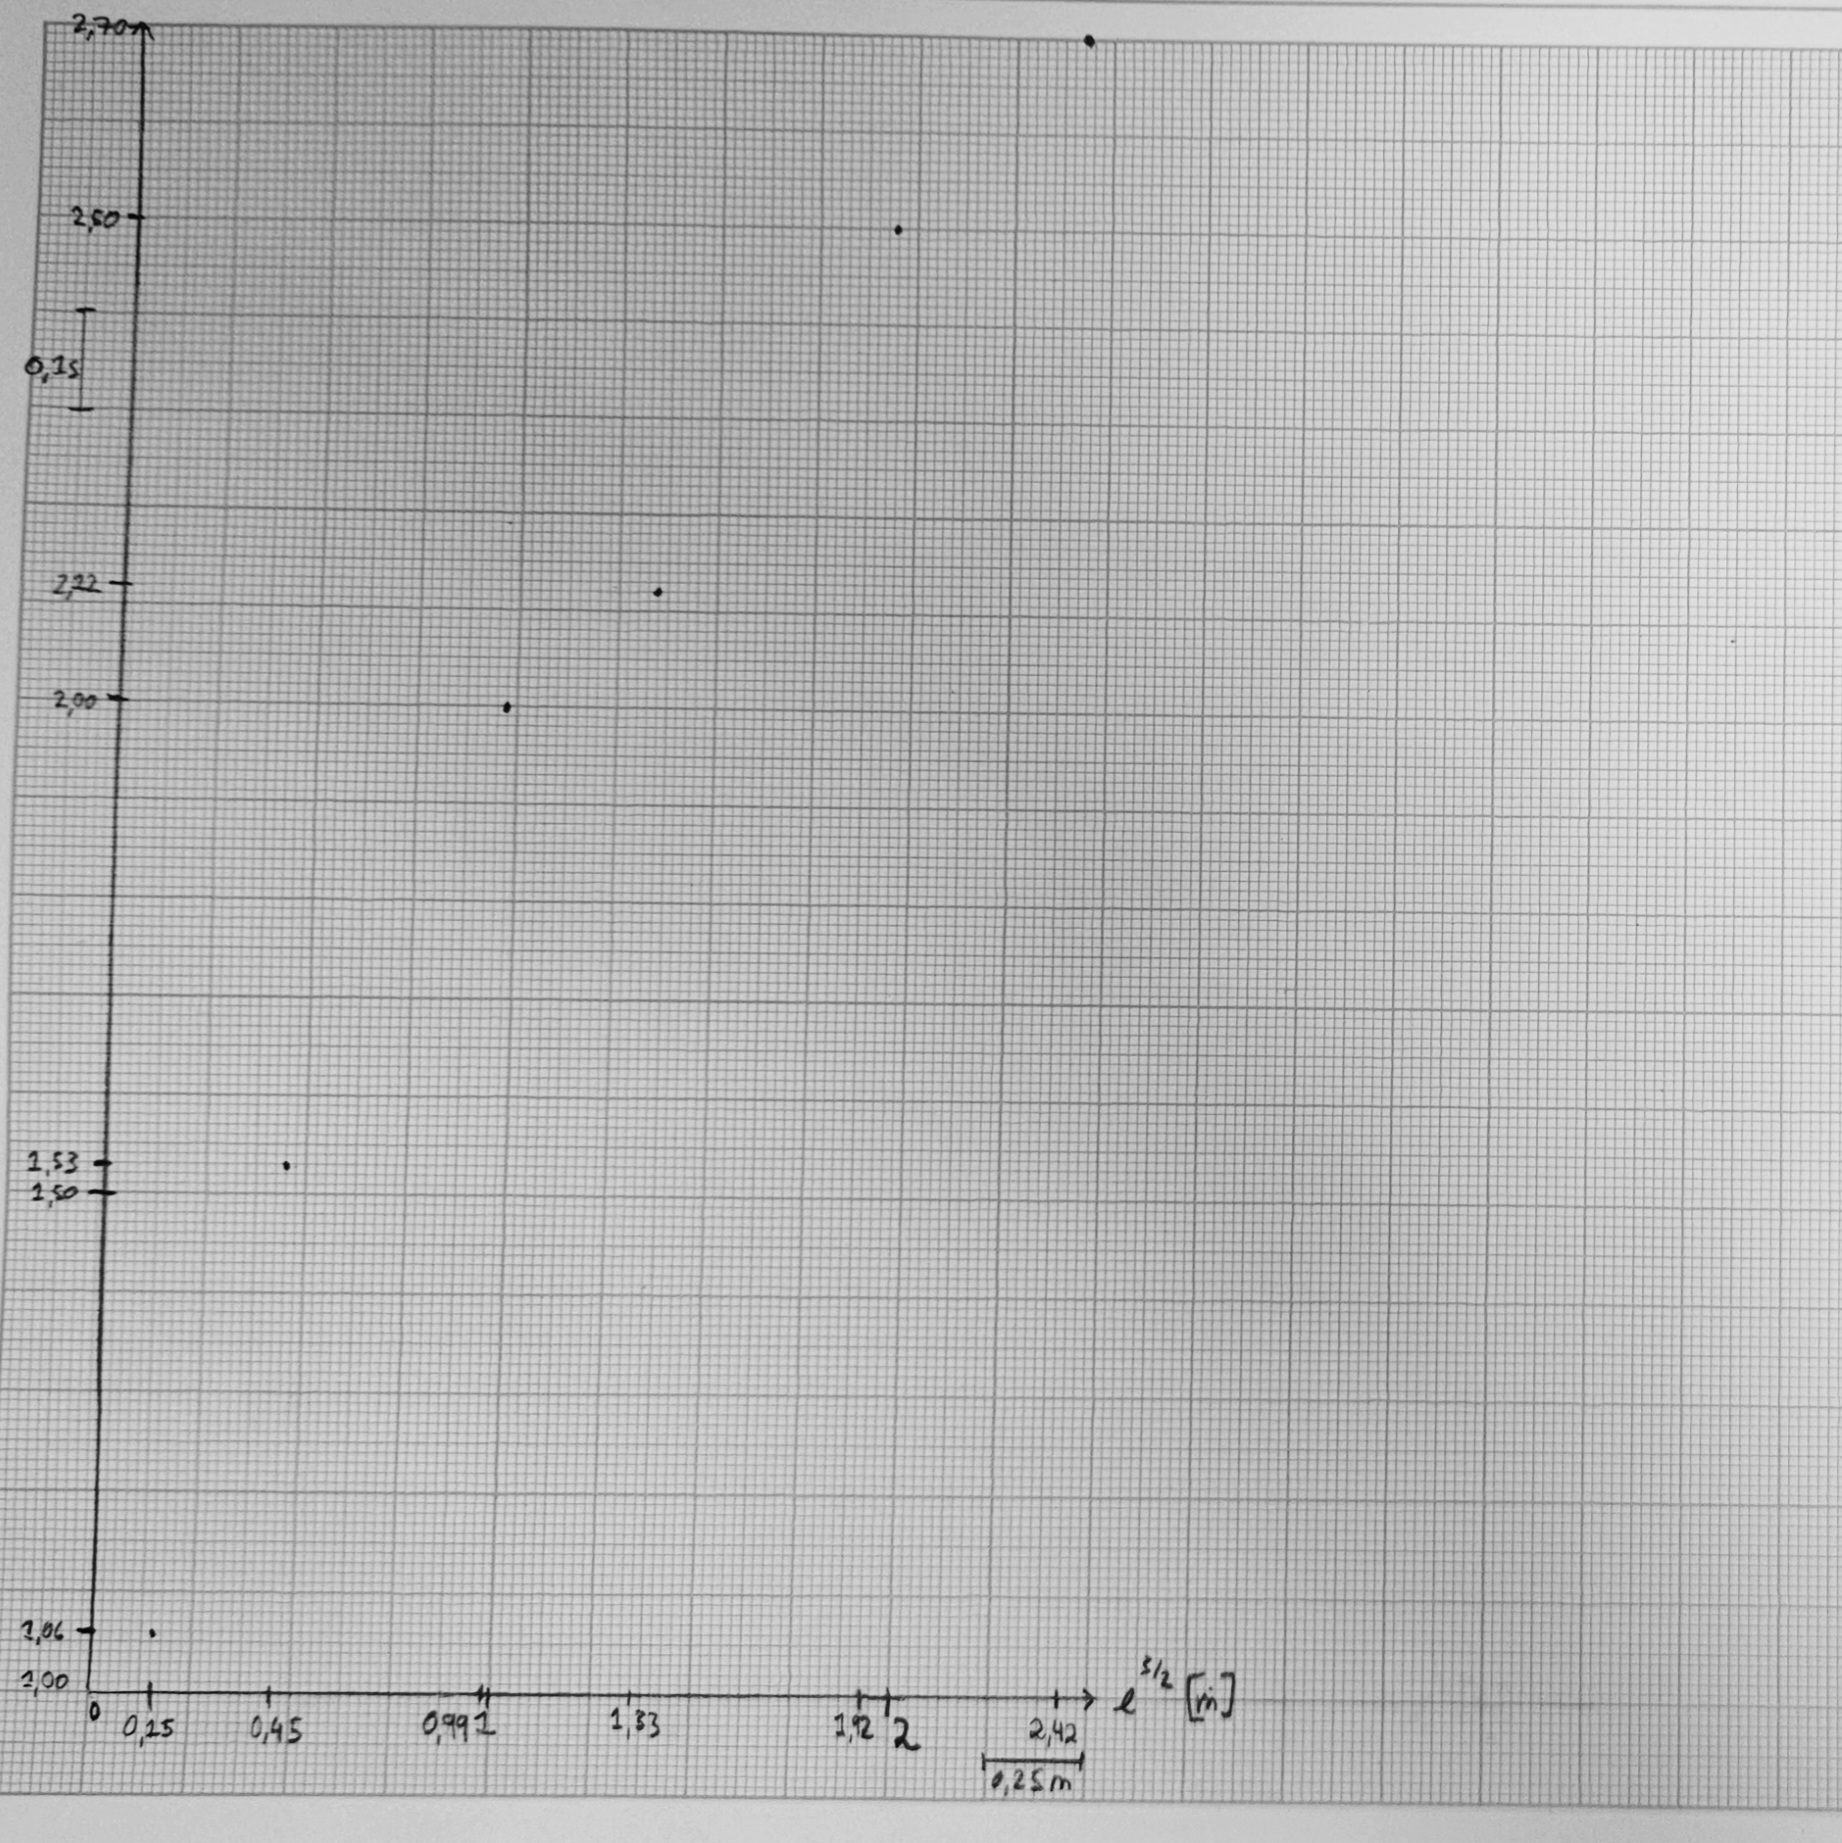
\includegraphics[width=0.75\textwidth]{fotopendolo/lunghezza32.jpg}
    \caption{Grafico $T$ vs $l^{3/2}$}
\end{figure}

\begin{figure}[!h]
    \centering
    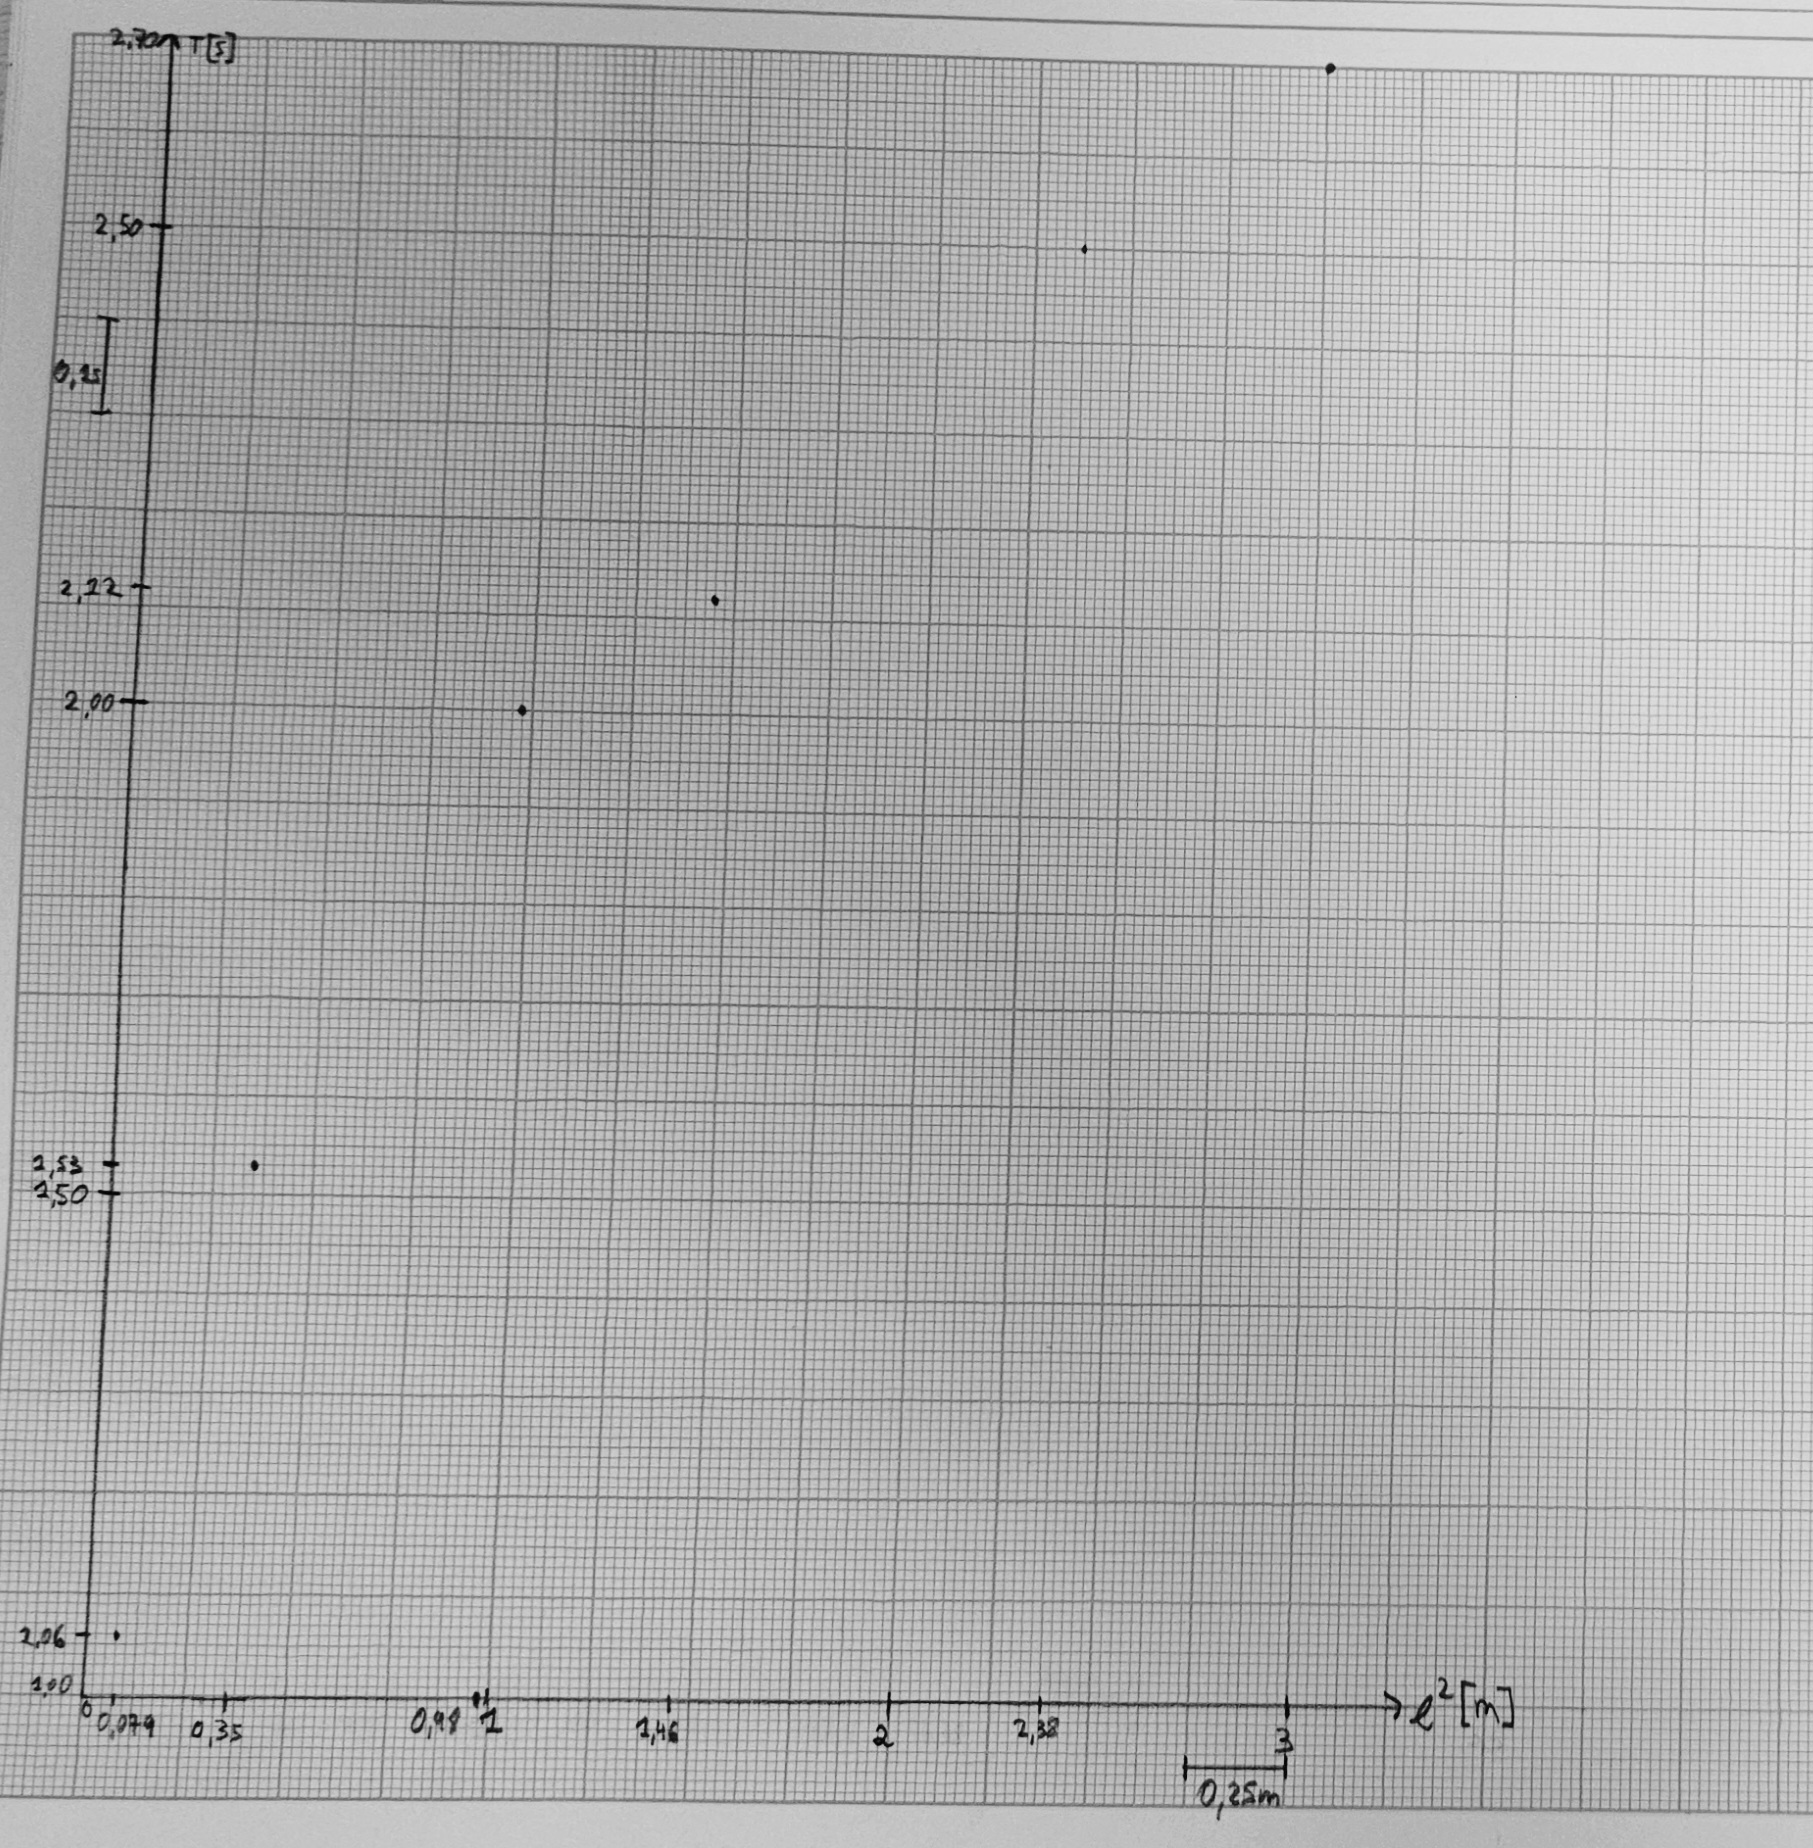
\includegraphics[width=0.75\textwidth]{fotopendolo/lunghezza21.jpg}
    \caption{Grafico $T$ vs $l^2$}
\end{figure}
\begin{figure}[!h]
    \centering
    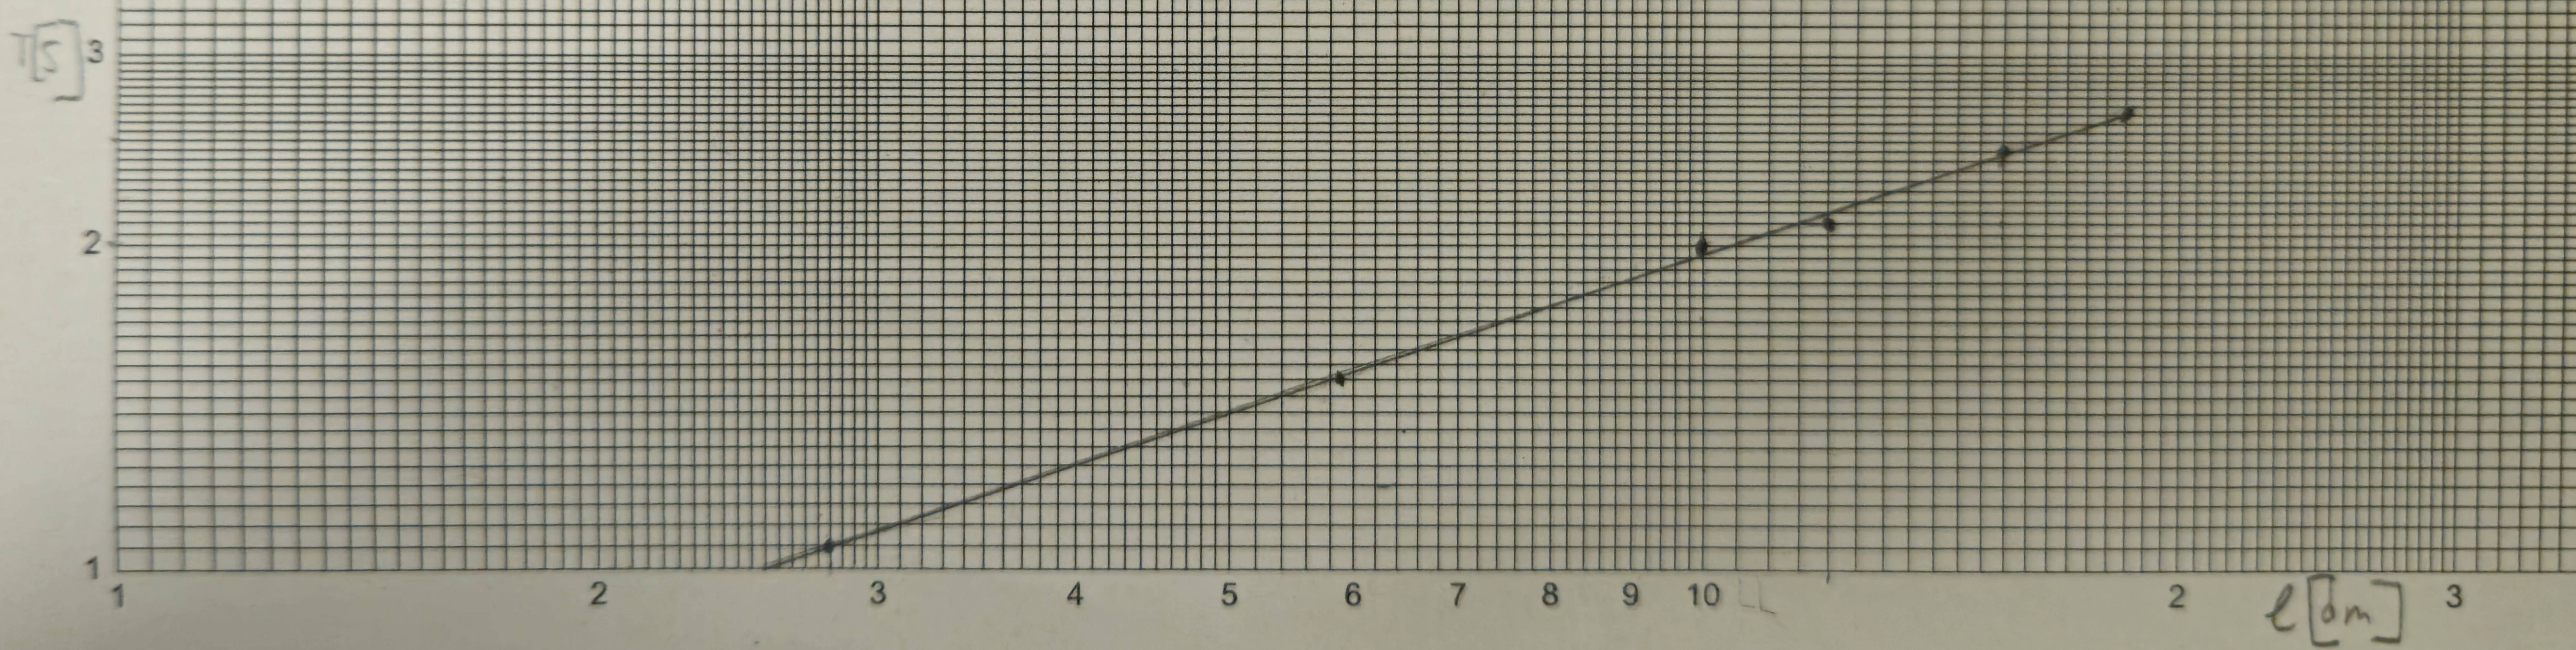
\includegraphics[width=\textwidth]{fotopendolo/loglog.jpg}
    \caption{$T$ in funzione di $l$ su carta logaritmica}
\end{figure}


\newpage
\subsubsection{Altri grafici}
\begin{figure}[!h]
    \centering
    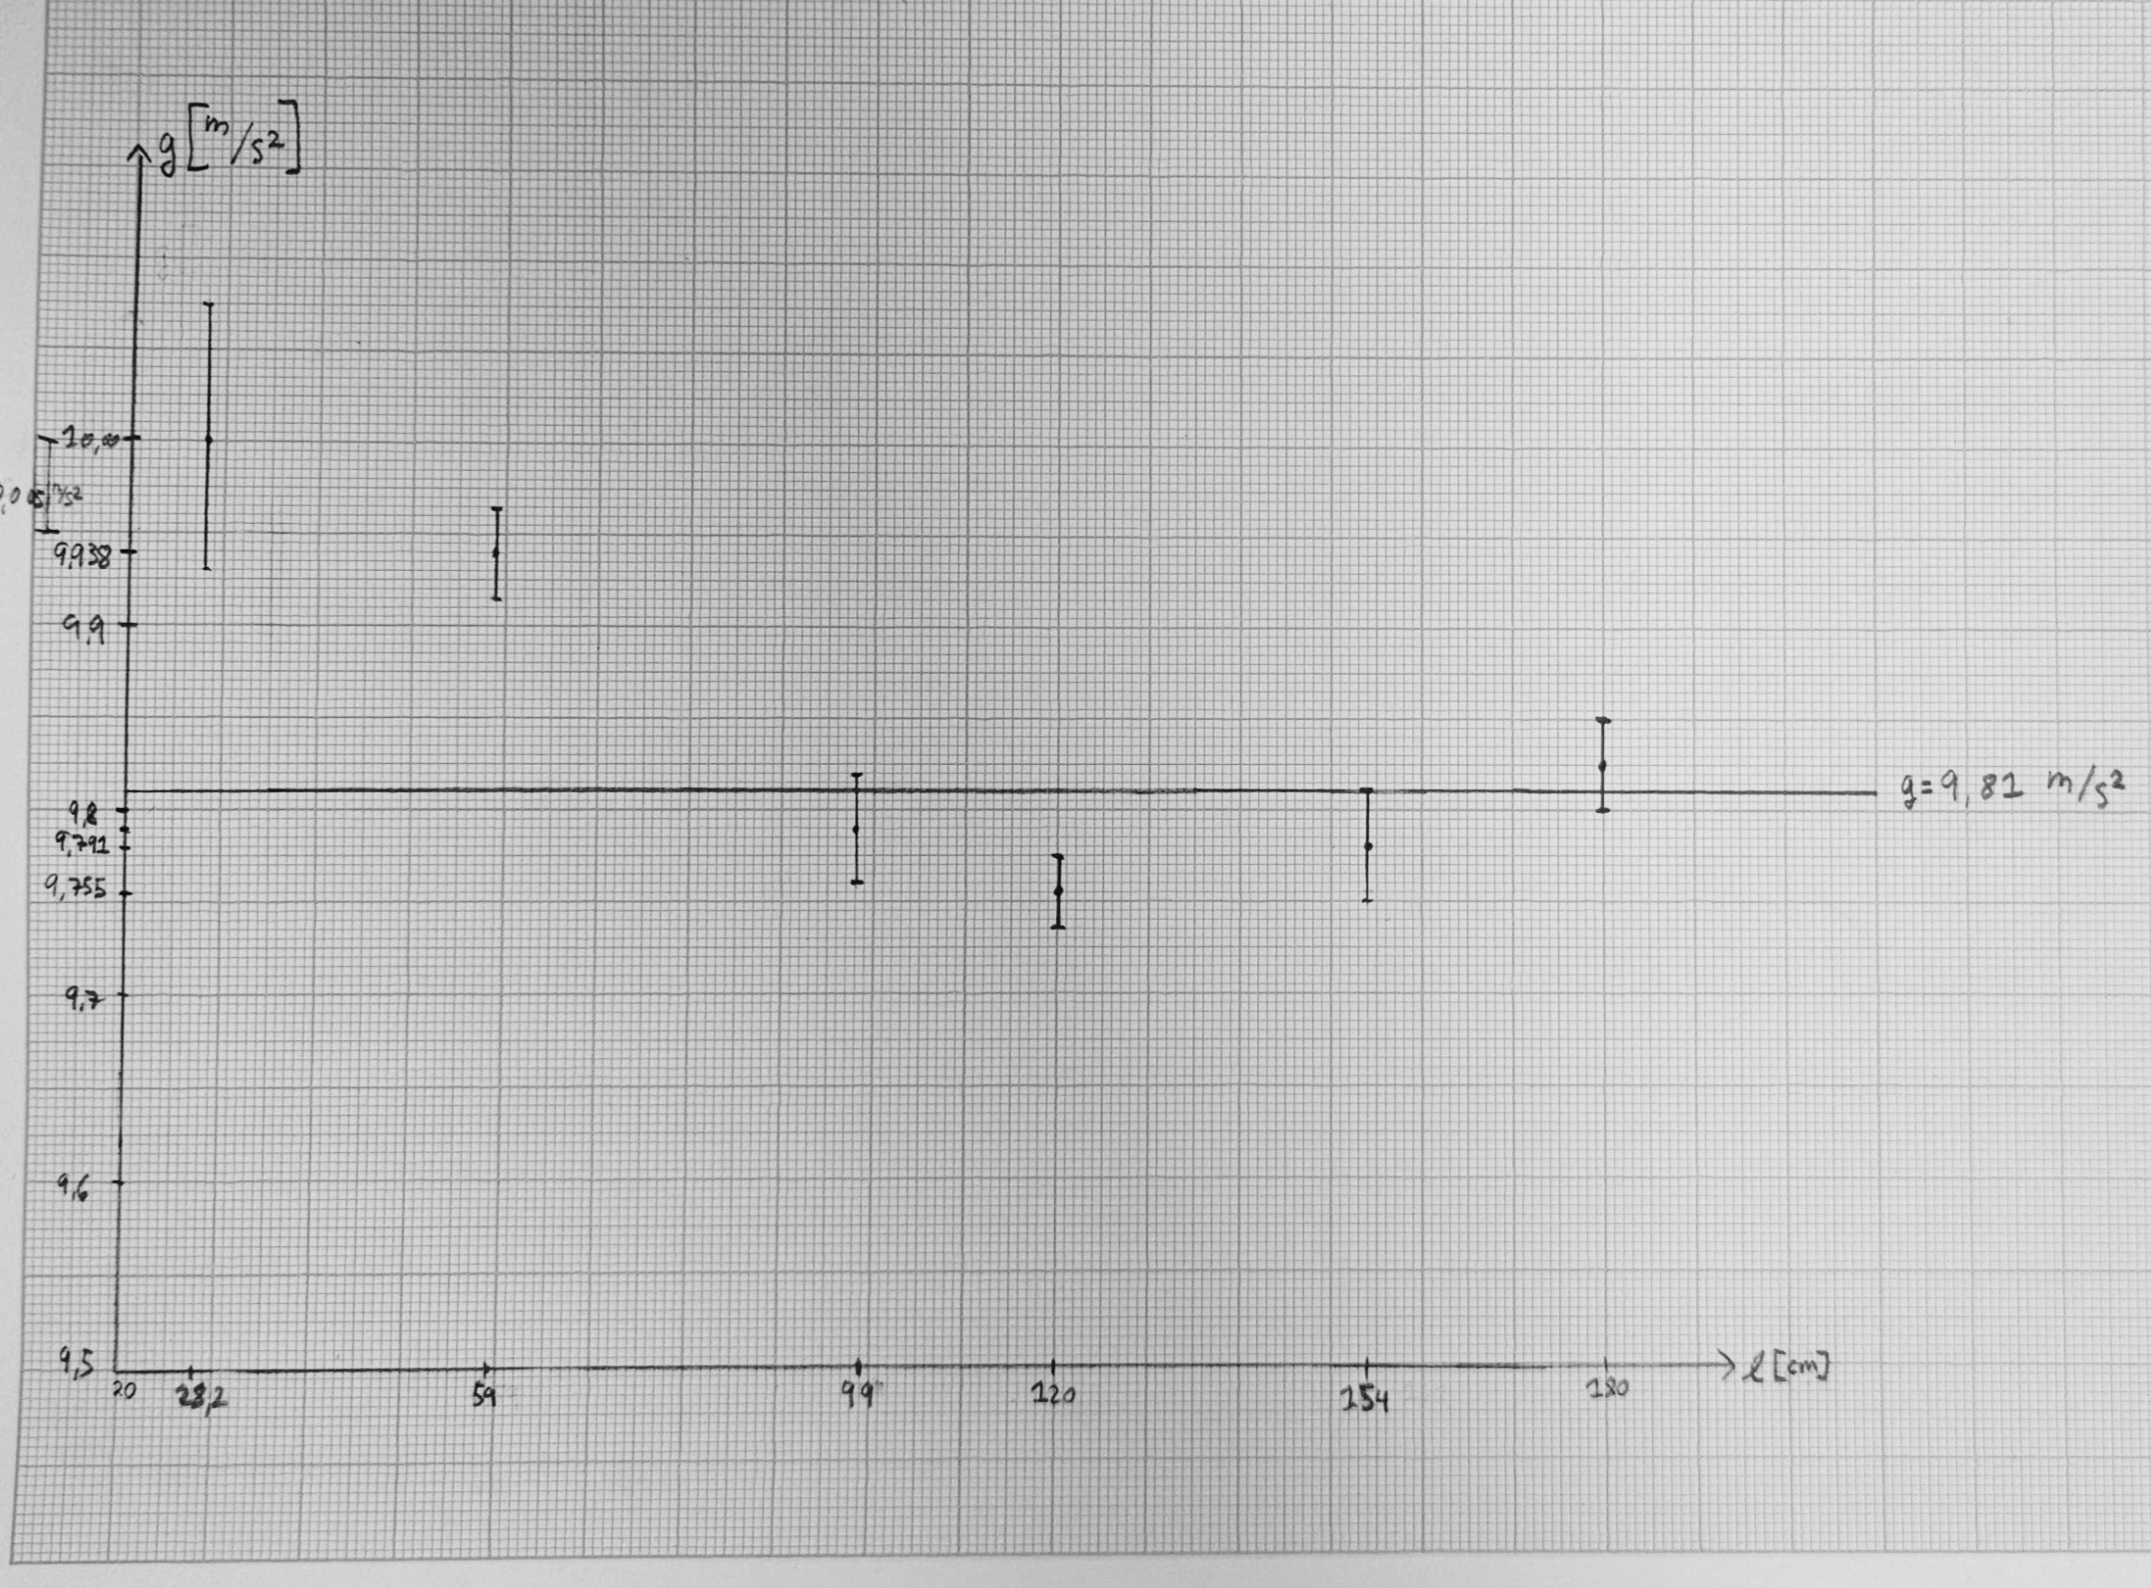
\includegraphics[width=0.75\textwidth]{fotopendolo/confrontog.jpg}
    \caption{Grafico dei valori di $g$}
\end{figure}

\begin{figure}[!h]
    \centering
    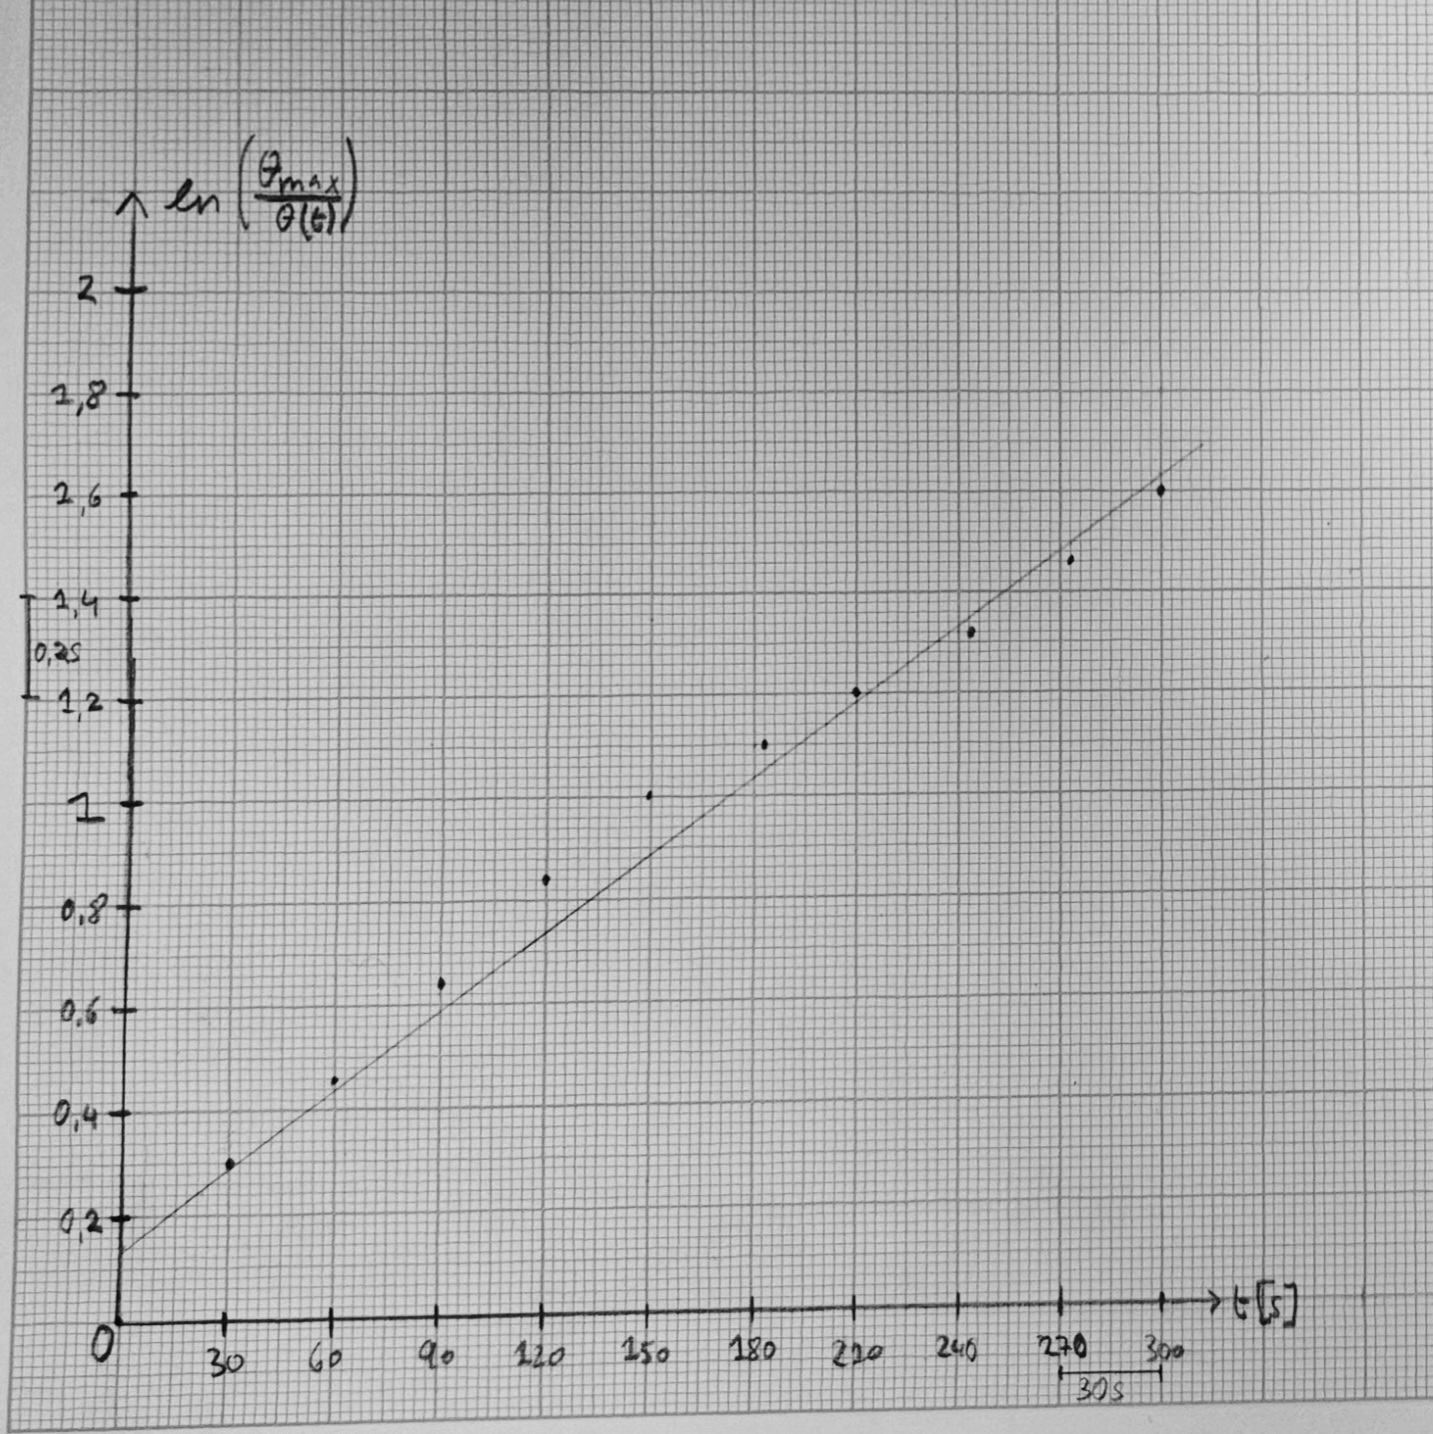
\includegraphics[width=0.75\textwidth]{fotopendolo/lunghezzalog.jpg}
    \caption{Grafico $T$ vs $ln\frac{\theta_{max}}{\theta(t)}$}
\end{figure}

\begin{figure}[!ht]
    \centering
    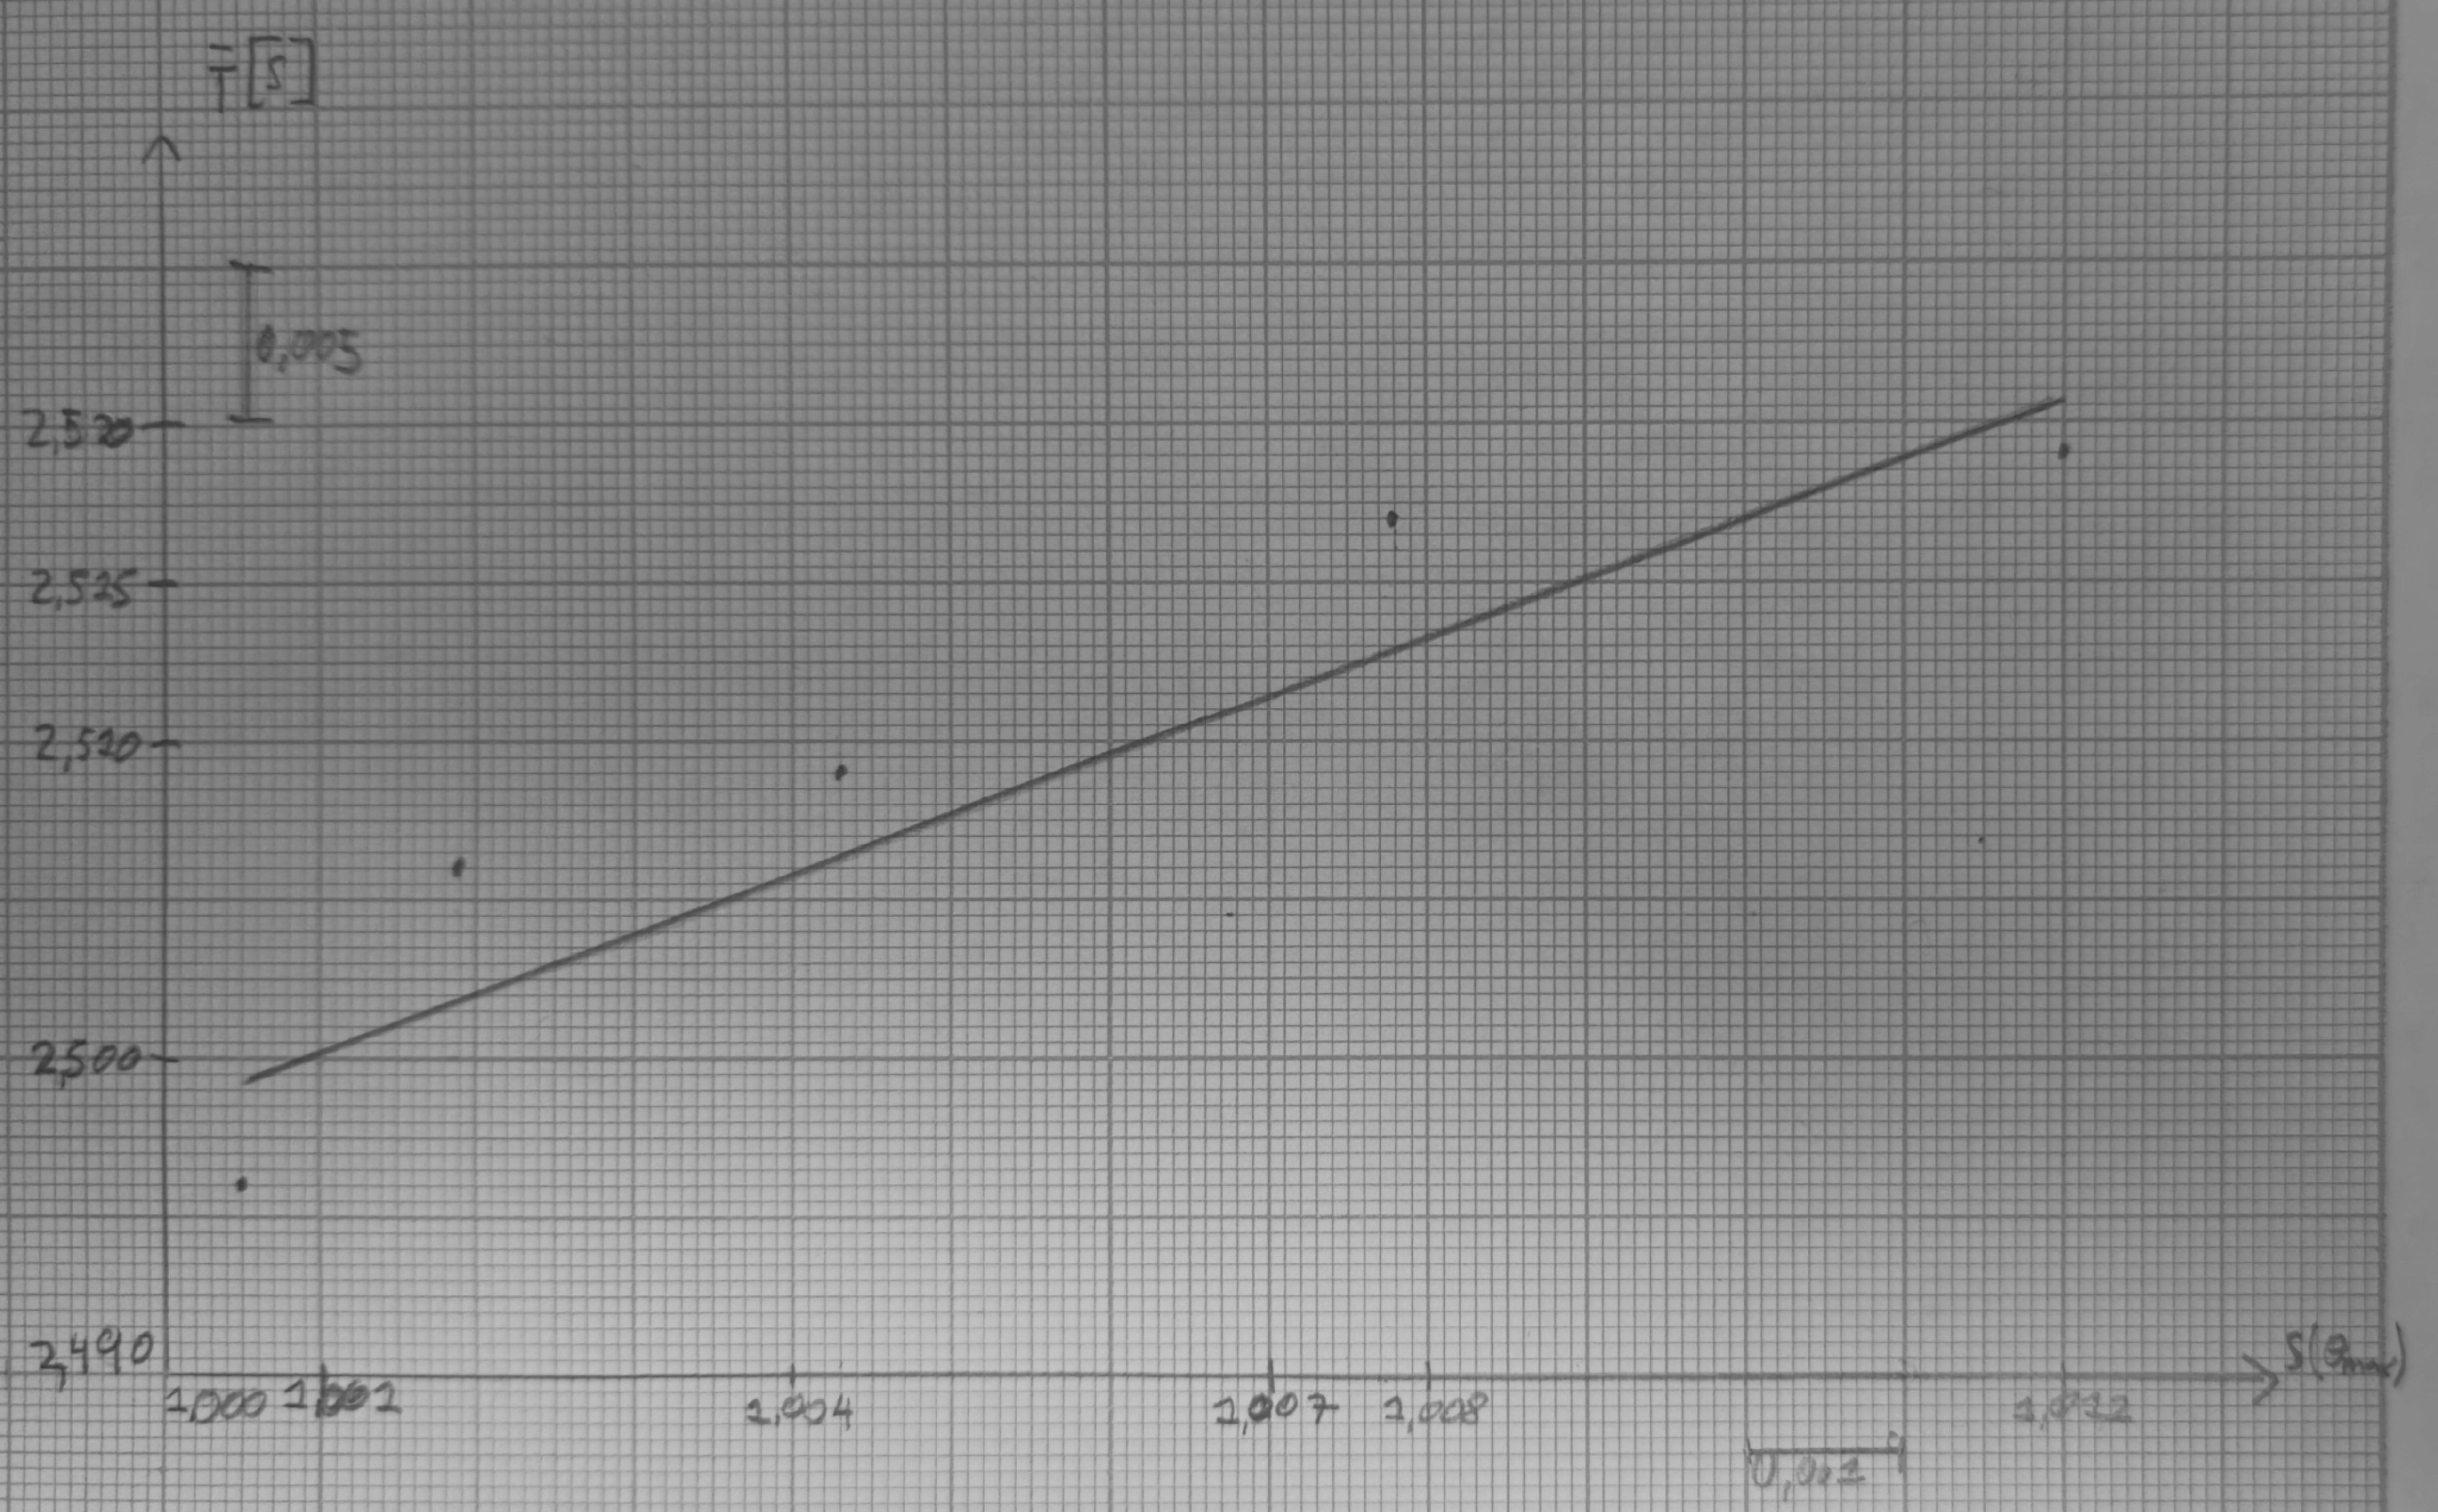
\includegraphics[width=\textwidth]{fotopendolo/attrito.jpg}
    \caption{Grafico di $S(\theta_{max}) vs \bar{T}$}
\end{figure}

\end{document}
